% Copyright (c) 2021 Robert Ryszard Paciorek <rrp@opcode.eu.org>
% 
% MIT License
% 
% Permission is hereby granted, free of charge, to any person obtaining a copy
% of this software and associated documentation files (the "Software"), to deal
% in the Software without restriction, including without limitation the rights
% to use, copy, modify, merge, publish, distribute, sublicense, and/or sell
% copies of the Software, and to permit persons to whom the Software is
% furnished to do so, subject to the following conditions:
% 
% The above copyright notice and this permission notice shall be included in all
% copies or substantial portions of the Software.
% 
% THE SOFTWARE IS PROVIDED "AS IS", WITHOUT WARRANTY OF ANY KIND, EXPRESS OR
% IMPLIED, INCLUDING BUT NOT LIMITED TO THE WARRANTIES OF MERCHANTABILITY,
% FITNESS FOR A PARTICULAR PURPOSE AND NONINFRINGEMENT. IN NO EVENT SHALL THE
% AUTHORS OR COPYRIGHT HOLDERS BE LIABLE FOR ANY CLAIM, DAMAGES OR OTHER
% LIABILITY, WHETHER IN AN ACTION OF CONTRACT, TORT OR OTHERWISE, ARISING FROM,
% OUT OF OR IN CONNECTION WITH THE SOFTWARE OR THE USE OR OTHER DEALINGS IN THE
% SOFTWARE.

\documentclass{pdfBooklets}

\title{Podstawy „elektryki”}
\author{%
	Robert Ryszard Paciorek\\\normalsize\ttfamily <rrp@opcode.eu.org>
}
\date  {2021-07-31}

\makeatletter\hypersetup{
	pdftitle = {\@title}, pdfauthor = {\@author}
}\makeatother

% Copyright (c) 2019-2020 Robert Ryszard Paciorek <rrp@opcode.eu.org>
% 
% MIT License
% 
% Permission is hereby granted, free of charge, to any person obtaining a copy
% of this software and associated documentation files (the "Software"), to deal
% in the Software without restriction, including without limitation the rights
% to use, copy, modify, merge, publish, distribute, sublicense, and/or sell
% copies of the Software, and to permit persons to whom the Software is
% furnished to do so, subject to the following conditions:
% 
% The above copyright notice and this permission notice shall be included in all
% copies or substantial portions of the Software.
% 
% THE SOFTWARE IS PROVIDED "AS IS", WITHOUT WARRANTY OF ANY KIND, EXPRESS OR
% IMPLIED, INCLUDING BUT NOT LIMITED TO THE WARRANTIES OF MERCHANTABILITY,
% FITNESS FOR A PARTICULAR PURPOSE AND NONINFRINGEMENT. IN NO EVENT SHALL THE
% AUTHORS OR COPYRIGHT HOLDERS BE LIABLE FOR ANY CLAIM, DAMAGES OR OTHER
% LIABILITY, WHETHER IN AN ACTION OF CONTRACT, TORT OR OTHERWISE, ARISING FROM,
% OUT OF OR IN CONNECTION WITH THE SOFTWARE OR THE USE OR OTHER DEALINGS IN THE
% SOFTWARE.

\usepackage{tikzPackets}
\usetikzlibrary{positioning} % for positionig nodes with `right = of X`
\usetikzlibrary{arrows.meta, decorations.markings} % for arrows formating in tikzpicture

\ifdefined\inputOnlyContent\else
	% redefine looks of footnotes to:
	%   margin (3mm), number (with constant filed width 6mm), empty space (remained from number filed width), text
	\makeatletter\renewcommand{\@makefntext}[1]{%
		\setlength{\@tempdima}{\columnwidth}\addtolength{\@tempdima}{-9mm}%
		\protect\footnotesize\hspace{1mm}\makebox[4mm][l]{\@thefnmark.}\parbox[t]{\@tempdima}{#1}%
	}\makeatother
\fi

\newcommand{\inputSideBySide}[4]{
\noindent
\begin{varwidth}[t]{9.3cm}
	\begin{center}
		#1:
	\end{center}
	\vspace{-0.35cm}
	\begin{adjustbox}{scale=.561}\inputFileContent{
		#2
	}\end{adjustbox}
\end{varwidth}
\hspace{0.4cm}
\begin{varwidth}[t]{9.3cm}
	\begin{center}
		#3:
	\end{center}
	\vspace{-0.35cm}
	\begin{adjustbox}{scale=.561}\inputFileContent{
		#4
	}\end{adjustbox}
\end{varwidth}
}

\newcommand{\inputSideBySideAsFigure}[6]{
\begin{figure}[h!]\label{#6}\inputSideBySide
	{#1}{#2}
	{#3}{#4}
	\caption{#5}
\end{figure}
}

\newcommand{\inputSingleAsFigure}[4][1.0]{
\begin{figure}[h!]\label{#4}
	\begin{center}\begin{adjustbox}{scale=#1}
		\inputFileContent{#2}
	\end{adjustbox}\end{center}
	\caption{#3}
\end{figure}
}


\begin{document}

\maketitle

% Copyright (c) 2018-2020 Matematyka dla Ciekawych Świata (http://ciekawi.icm.edu.pl/)
% Copyright (c) 2018-2020 Robert Ryszard Paciorek <rrp@opcode.eu.org>
% 
% MIT License
% 
% Permission is hereby granted, free of charge, to any person obtaining a copy
% of this software and associated documentation files (the "Software"), to deal
% in the Software without restriction, including without limitation the rights
% to use, copy, modify, merge, publish, distribute, sublicense, and/or sell
% copies of the Software, and to permit persons to whom the Software is
% furnished to do so, subject to the following conditions:
% 
% The above copyright notice and this permission notice shall be included in all
% copies or substantial portions of the Software.
% 
% THE SOFTWARE IS PROVIDED "AS IS", WITHOUT WARRANTY OF ANY KIND, EXPRESS OR
% IMPLIED, INCLUDING BUT NOT LIMITED TO THE WARRANTIES OF MERCHANTABILITY,
% FITNESS FOR A PARTICULAR PURPOSE AND NONINFRINGEMENT. IN NO EVENT SHALL THE
% AUTHORS OR COPYRIGHT HOLDERS BE LIABLE FOR ANY CLAIM, DAMAGES OR OTHER
% LIABILITY, WHETHER IN AN ACTION OF CONTRACT, TORT OR OTHERWISE, ARISING FROM,
% OUT OF OR IN CONNECTION WITH THE SOFTWARE OR THE USE OR OTHER DEALINGS IN THE
% SOFTWARE.

Python jest wysokopoziomowym językiem programowania ogólnego przeznaczenia.
Oznacza to że jego składnia została tak zbudowana aby maksymalizować czytelność kodu dla człowieka i być niezależna od sprzętowych i implementacyjnych detali
	oraz że nie ma pojedynczego dedykowanego obszaru zastosowań (z łatwością może być stosowany do różnych zastosowań).

Wsórd cech i zalet Pythona należy wymienić:
\begin{itemize}
\item jest językiem interpretowanym\footnote{może być i w niektórych sytuacjach podlega kompilacji do kodu pośredniego celem zwiększenia wydajności}, co daje łatwiejsze modyfikowanie kodu, eksperymentowanie z nim, itd
\item jest jednym z najpopularniejszych języków programowania (wg niektórych źródeł nawet najpopularniejszym), więc nie jest "dydaktyczną egzotyką", która potem do niczego się nie przyda
\item działa na wielu różnych platformach sprzętowych i na różnych systemach oparacyjnych
\item istnieje bardzo wiele bibliotek pythonowych (posiadających pythonowe API), a można korzystać także z "niedostosowanych" do Pythona bibliotek C (.so, .dll)
\item jest łatwo rozszerzalny przy pomocy (własnych) bibliotek/modułów tworzonych w C/C++ (podstawowy interpreter napisany jest C)
\item kod pythonowy może być łatwo wywoływany z poziomu C/C++, co pozwala na łatwe wykorzystanie Pythona jako języka skryptowego dla projektów tworzonych w C/C++
\end{itemize}

Ponadto Python jest wygodniejszy w uczeniu od wielu innych języków m.in. ze względu na to że
	kod pythonowy realizujący tą samą funkcjonalność, przy takim samym poziomie obsługi błędów, etc i podobnej czytelności,
	praktycznie zawsze jest krótszy od kodu C (a potrafi być krótszy kilkukrotnie, więc łatwiej go pokazać i omówić).

W ramach kursu zajmować się będziemy językiem Python w wersji 3 (czyli o pełnym numerze zaczynającym się od 3, np. 3.7.1).
Należy o tym pamiętać i zwracać na to uwagę, gdyż wersja ta różni się na tyle znacząco w stosunku co do starszej, lecz wciąż używanej wersji 2,
	że programy, prezentowane w tym skrypcie i te które będziemy pisać na zajęciach nie będą działać w drugiej wersji Pythona.

% Copyright (c) 2015-2021 Robert Ryszard Paciorek <rrp@opcode.eu.org>
% 
% MIT License
% 
% Permission is hereby granted, free of charge, to any person obtaining a copy
% of this software and associated documentation files (the "Software"), to deal
% in the Software without restriction, including without limitation the rights
% to use, copy, modify, merge, publish, distribute, sublicense, and/or sell
% copies of the Software, and to permit persons to whom the Software is
% furnished to do so, subject to the following conditions:
% 
% The above copyright notice and this permission notice shall be included in all
% copies or substantial portions of the Software.
% 
% THE SOFTWARE IS PROVIDED "AS IS", WITHOUT WARRANTY OF ANY KIND, EXPRESS OR
% IMPLIED, INCLUDING BUT NOT LIMITED TO THE WARRANTIES OF MERCHANTABILITY,
% FITNESS FOR A PARTICULAR PURPOSE AND NONINFRINGEMENT. IN NO EVENT SHALL THE
% AUTHORS OR COPYRIGHT HOLDERS BE LIABLE FOR ANY CLAIM, DAMAGES OR OTHER
% LIABILITY, WHETHER IN AN ACTION OF CONTRACT, TORT OR OTHERWISE, ARISING FROM,
% OUT OF OR IN CONNECTION WITH THE SOFTWARE OR THE USE OR OTHER DEALINGS IN THE
% SOFTWARE.

\section{Obwody prądu zmiennego}

W elektronice (zwłaszcza analogowej) spotyka się z obwodami prądu zmiennego, jednak są to na ogół sygnały zmienne i wartość płynącego prądu (a co za tym idzie także mocy) nie jest znaczna. Inaczej sytuacja wygląda w instalacjach elektrycznych gdzie typowo mamy prąd przemienny (50Hz lub 60Hz, zależnie od rejonu świata) oraz spore wartości napięcia, prądy i moce. W związku z tym spojrzenie elektryka jest trochę inne niż elektronika – nie ma np. większego znaczenia pasmo częstotliwości danego układu, a istotne jest przesuniecie fazowe pomiędzy prądem a napięciem oraz związane z tym zagadnienia mocy biernej i pozornej.

\subsection{Wartość szytowa, międzyszczytowa, skuteczna i amplituda}

\begin{center} \begin{adjustbox}{scale=1.0} \begin{tikzpicture}
	\begin{axis}[
		axis lines=middle,
		unit vector ratio*=1 1,
		scale=2.3,
		ymin=-1.9, ymax=1.9, xmin=-3.5, xmax=7,
		domain=-3.5:7,
		samples=100,
		ymajorticks=false,
		xmajorticks=false,
		disabledatascaling
	]
	\addplot [mark=none] {sin(deg(x))};
	
	\draw[dashed] (-pi, 1)  -- (2*pi, 1);
	\draw[dashed] (-pi, 0.7071)  -- (2*pi, 0.7071);
	\draw[dashed] (-pi, -1) -- (2*pi, -1);
	
	\draw[<->, line width=0.35mm, green] (-0.5*pi, -1) -- (-0.5*pi, 1);
	\node[anchor = south, align = center, green] at (-0.5*pi, 1.0) {wartość międzyszczytowa\\\textit{peak to peak}};
	
	\draw[<->, line width=0.35mm, blue] (0.5*pi, 0) -- (0.5*pi, 1);
	\node[anchor = south, align = center, blue] at (0.5*pi, 1.0) {wartość szczytowa\\\textit{peak}};
	
	\draw[<->, line width=0.35mm, red] (1.5*pi, 0) -- (1.5*pi, 0.7071);
	\node[anchor = south, align = center, red] at (1.5*pi, 1.0) {wartość skuteczna\\\textit{RMS}};
	
	\draw[purple, dashed] (0, 0) -- (0, -1.6);
	\draw[purple, dashed] (2*pi, 0) -- (2*pi, -1.6);
	\draw[<->, purple]    (0, -1.3) -- node[below] {okres $T = 1/f$} (2*pi, -1.3);
\end{axis}
\end{tikzpicture} \end{adjustbox} \end{center} \vspace{-0.3cm}

\subsubsection{Wartość międzyszczytowa (peak to peak)}

Wartość międzyszczytowa jest to różnica pomiędzy wartością maksymalną a minimalną sygnału. Nie uwzględnia ona składowej stałej.

\subsubsection{Wartość szyszczytowa (peak)}

Maksymalna wartość sygnału względem poziomu odniesienia (np. zera lub poziomu składowej DC).
Zależnie od przyjętego poziomu odniesienia może uwzględniać, uwzględniać częściowo lub nie uwzględniać składowej stałej.

Dla symetrycznych przebiegów okresowych (takich jak sinusoidalny, prostokątny lub trójkątny) bez składowej stałej wartość szczytowa stanowi połowę wartości międzyszczytowej i jest równa \href{https://en.wikipedia.org/wiki/Amplitude}{\strong{amplitudzie}} sygnału. Jest to też maksymalna wartość napięcia uzyskanego w wyniku wyprostowania napięcia przemiennego\footnote{w rzeczywistości będzie pomniejszona o spadek napięcia na układzie prostującym}.

\subsubsection{Wartość skuteczna (RMS)}

\href{https://pl.wikipedia.org/wiki/Warto\%C5\%9B\%C4\%87_skuteczna}{Wartość skuteczna} $I_{sk}$ prądu przemiennego (opisanego funkcją $i(t)$) jest to wartość prądu stałego równoważnego mu pod względem wydzielenia takiej samej mocy w trakcie pełnego okresu.

\noindent
Moc prądu stałego wydzielana w czasie T: $$P = {I_{sk}}^2RT$$
Moc prądu przemiennego wydzielana w czasie pełnego okresu T: $$P = \int\limits^{T}_{0}{i^2(t)Rdt}$$
Z porównania otrzymujemy:

$$I_{sk} = \sqrt{\frac{1}{T}\int\limits^{T}_{0}{i^2(t)}dt}$$

\noindent
Analogicznie napięcie skuteczne:
$$U_{sk} = \sqrt{\frac{1}{T}\int\limits^{T}_{0}{u^2(t)}dt}$$

\noindent
Dla przebiegu sinusoidalnego:
	$$I_{sk} = \frac{I_{pp}}{2\sqrt{2}} = \frac{I_{0}}{\sqrt{2}} \qquad\qquad U_{sk} = \frac{U_{pp}}{2\sqrt{2}} = \frac{U_{0}}{\sqrt{2}}$$
gdzie:
\begin{itemize}
	\item $I_{pp}$ – wartość międzyszczytowa natężenia prądu
	\item $I_{0}$  – amplituda (wartość szytytowa) natężenia prądu
	\item $U_{pp}$ – wartość międzyszczytowa napięcia
	\item $U_{0}$  – amplituda (wartość szytytowa) napięcia
\end{itemize}

Ze względu na równoważność efektów z prądem stałym wartości skuteczne są powszechnie stosowane do opisywania prądów przemiennych.
Także mierniki elektryczne prądu przemiennego podają wartości skuteczne natężenia i napięcia\footnote{
	Mierniki nie \textit{true RMS} podają je z zależności $I_{sk} = \frac{I_{0}}{\sqrt{2}}$, $U_{sk} = \frac{U_{0}}{\sqrt{2}}$,
		która jest prawdziwa tylko dla przebiegu sinusoidalnego.
	Mierniki \textit{true RMS} dokonują obliczenia „rzeczywistej” wartości skutecznej wykonując odpowiednio wiele próbkowań sygnału.
}.


\subsection{Impedancja}

\href{https://pl.wikipedia.org/wiki/Impedancja}{Impedancja} jest uogólnieniem oporu dla obwodów prądu przemiennego zawierających kondensatory (pojemności) i cewki (indukcyjności). Jest to wartość zespolona dana zależnością:

$$Z = R + jX$$

\noindent
gdzie:
\begin{itemize}
	\item $R$ – \strong{rezystancja},
	\item $X$ – \strong{reaktancja}:
	\begin{itemize}
		\item dla cewki: $X = \omega L$
		\item dla kondensatora: $X = - \frac{1}{\omega C}$
		\item gdzie:
		\begin{itemize}
			\item $L$ – indukcyjność cewki
			\item $C$ – pojemność kondensatora
			\item $\omega = 2 \pi f$ – częstość kołowa
			\item $f$ to częstotliwość prądu (w Hz)
		\end{itemize}
	\end{itemize}
	\item j – jedność urojona, $j^2 = -1$
\end{itemize}

\vspace{5mm}\noindent
Należy zwrócić uwagę na przeciwny znak reaktancji dla pojemności i indukcyjności.
Jest to związane ze znoszeniem się reaktancji (a zatem też impedancji) połączonych ze sobą kondensatora i cewki.
W związku z tym impedancja może mieć charakter pojemnościowy (gdy $X<0$), indukcyjny (gdy $X>0$)\footnote{
	w odbu wypadkach z możliwą jakąś wartością rezystancji
} lub czysto rezystancyjny (gdy $X=0$, czyli $Z=R$).

\begin{center} \begin{adjustbox}{scale=1.0} \begin{tikzpicture}
	\tikzstyle{invisibleNode}=[inner sep=0, outer sep = 0pt, minimum size=0]
	\begin{axis}[
		axis lines=middle,
		xlabel=$Re$,
		xmin=-1.5, xmax=3.5,
		xtick={      -1,   1},
		xlabel style={above, xshift=-1ex},
		ylabel=$Im$,
		ymin=-3.0, ymax=3.0,
		yticklabels={$-i$, $i$},
		ytick={      -1,   1},
		disabledatascaling
	]
		\node[invisibleNode] at (2.5,1.8) (Z) {};
		
		\draw[->, >={Stealth[length=8pt,width=6pt]}] (0,0) -- node[above] {$Z$} (Z);
		
		\draw[blue, dashed] (Z) -- (Z |- 0,0);
		\node[blue, anchor = north] at (Z |- 0,0) {R};
		
		\draw[red, dashed] (Z) -- (Z -| 0,0);
		\node[red, anchor = east] at (Z -| 0,0) {X};
		
		\draw ([shift=(0:1.3)]0,0) arc (0:36:1.3);
		\node at (0.9, 0.27) {$\phi$};
		
		\node[align=center] at (1.75, -2) {\small $Z$ ma charkter\\indukcyjny};
	\end{axis}
\end{tikzpicture} \end{adjustbox} \hspace{0.5cm} \begin{adjustbox}{scale=1.0} \begin{tikzpicture}
	\tikzstyle{invisibleNode}=[inner sep=0, outer sep = 0pt, minimum size=0]
	\begin{axis}[
		axis lines=middle,
		xlabel=$Re$,
		xmin=-1.5, xmax=3.5,
		xtick={      -1,   1},
		xticklabel style={above, yshift=0.5ex},
		xlabel style={below, xshift=-1ex},
		ylabel=$Im$,
		ymin=-3.0, ymax=3.0,
		yticklabels={$-i$, $i$},
		ytick={      -1,   1},
		disabledatascaling
	]
		\node[invisibleNode] at (2.5,-1.8) (Z) {};
		
		\draw[->, >={Stealth[length=8pt,width=6pt]}] (0,0) -- node[below] {$Z$} (Z);
		
		\draw[blue, dashed] (Z) -- (Z |- 0,0);
		\node[blue, anchor = south] at (Z |- 0,0) {R};
		
		\draw[red, dashed] (Z) -- (Z -| 0,0);
		\node[red, anchor = east] at (Z -| 0,0) {X};
		
		\draw ([shift=(0:1.3)]0,0) arc (0:-36:1.3);
		\node at (0.9, -0.27) {$\phi$};
		
		\node[align=center] at (1.75, 1.5) {\small $Z$ ma charkter\\pojemnościowy};
	\end{axis}
\end{tikzpicture} \end{adjustbox} \end{center} \vspace{-0.3cm}

\subsubsection{łączenie szeregowe i równoległe}

Impedancja zastępcza połączenia \strong{szeregowego} dana jest zależnością: $$Z = Z_1 + Z_2$$
Impedancja zastępcza połączenia \strong{równoległego} dana jest zależnością: $$\frac{1}{Z} = \frac{1}{Z_1} + \frac{1}{Z_2}$$

\noindent
Jest to zasadniczo sumowanie wektorów / odwrotności wektorów\footnote{
	dla $Z = R + jX$ mamy $\sfrac{1}{Z} = \sfrac{(R - jX)}{|Z|^2}$
} na płaszczyźnie zespolonej.

\subsubsection{moduł impedancji (zawada)}

$$|Z| = \sqrt{R^2 + X^2}$$


\subsection{Szeregowy obwód RLC}

Wiele odbiorników elektrycznych (np. silniki, zasilacze komputerowy, itd.) podłączonych do instalacji zasilającej prądu przemiennego posiada niezerową reaktancja, czyli stanowi obciążenie indukcyjne albo pojemnościowe. Rozważmy zatem przypadek szeregowo połączonych elementów reprezentujących rezystancję, pojemność i indukcyjność\footnote{
	Nie ma sensu zastanawiania się nad realnym układem połączenia tych elementów wewnątrz urządzenia
		– każde urządzenie można przedstawić jako szeregowo połączoną jakąś rezystancję zastępczą ($\ge 0$)
		z jakąś reaktancją zastępczą (o charakterze pojemnościowym albo indukcyjnym – w naszych rozważaniach będziemy mieć albo pojemność albo indukcję).
	I właśnie jako na takie wartości zastępcze (mogące zależeć od całego zestawu realnych rezystancji pojemności i indukcyjności) należy patrzyć na wartości R, L i C występujące w dalszych obliczeniach. Przy czym wystąpienie pojemności wyklucza wystąpienie indukcyjności i na odwrót.
}.


\subsubsection{Natężenie prądu}

$$I_{sk} = U_{sk} / |Z| = U_{sk} / \sqrt{R^2 + \left(\omega L - { 1 \over \omega C}\right)^2}$$

\noindent
gdzie:
\begin{itemize}
	\item $U_{sk}$, $I_{sk}$ - wartości skuteczne napięcia i prądu
	\item $L = 0$ gdy charakter pojemnościowy\footnote{
		zastępcza reaktancja ujemna, na co można patrzeć jako na brak cewki (zastąpienie jej zwarciem) w szeregowym połączeniu RLC
	}, lub $C = \infty$ gdy charakter indukcyjny\footnote{
		zastępcza reaktancja dodatnia, na co można patrzeć jako na brak kondensatora (zastąpiony go zwarciem) w szeregowym połączeniu RLC
	}
\end{itemize}

\subsubsection{Kąt przesunięcia fazowego}

$$\phi = \arctan \left({X_L + X_C \over R}\right) = \arctan \left({\omega L - \frac{1}{\omega C} \over R} \right)$$

\noindent
Jest to jednocześnie kąt pomiędzy $Z$ a osią rzeczywistą na płaszczyźnie zespolone, jak również kąt o który odsunięte są od siebie przebiegi napięcia i prądu.

\begin{center} \begin{adjustbox}{scale=1.0} 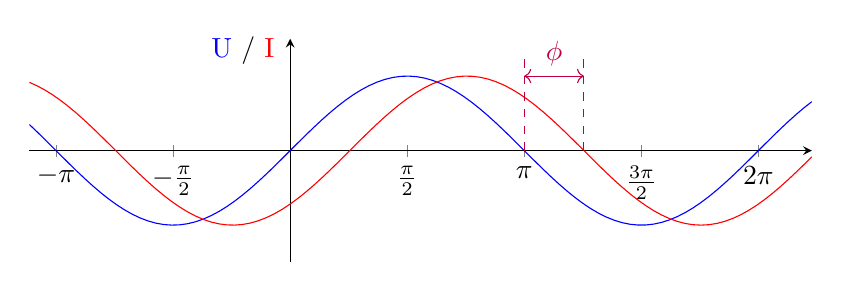
\begin{tikzpicture}
	\begin{axis}[
		axis lines=middle,
		unit vector ratio*=1 1,
		scale=1.45,
		ymin=-1.5, ymax=1.5, xmin=-3.5, xmax=7,
		domain=-3.5:7,
		samples=100,
		ylabel={\color{blue}U} / {\color{red}I},
		ylabel style={left, yshift=-1ex, xshift=-.5ex},
		ymajorticks=false,
		xtick={ -pi, -0.5*pi, 0.5*pi, pi, 1.5*pi, 2*pi},
		xticklabels={$-\pi$, $-\frac{\pi}{2}$, $\frac{\pi}{2}$, $\pi$, $\frac{3\pi}{2}$, $2\pi$},
		disabledatascaling
	]
	\addplot [mark=none, blue] {sin(deg(x))};
	\addplot [mark=none, red] {sin(deg(x-.8))};
	
	\draw[purple, dashed] (pi, 0) -- (pi, 1.3);
	\draw[purple, dashed] (pi+0.8, 0) -- (pi+0.8, 1.3);
	\draw[<->, purple]    (pi, 1) -- node[above] {$\phi$} (pi+0.8, 1);
\end{axis}
\end{tikzpicture} \end{adjustbox}
\\\strong{Obciążenie indukcyjne}: prąd wyprzedza napięcie, $\phi > 0$, $X > 0$
\end{center} \vspace{-0.3cm}

\begin{center} \begin{adjustbox}{scale=1.0} 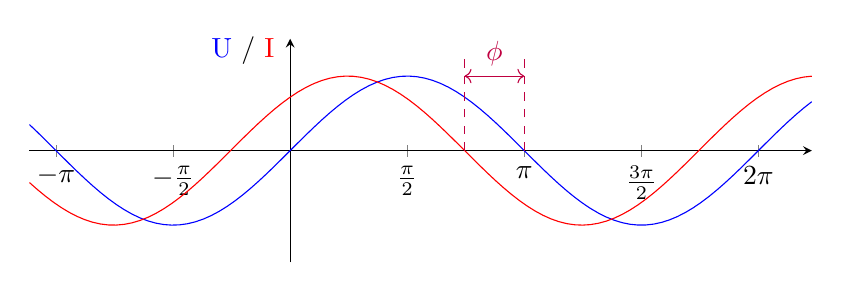
\begin{tikzpicture}
	\begin{axis}[
		axis lines=middle,
		unit vector ratio*=1 1,
		scale=1.45,
		ymin=-1.5, ymax=1.5, xmin=-3.5, xmax=7,
		domain=-3.5:7,
		samples=100,
		ylabel={\color{blue}U} / {\color{red}I},
		ylabel style={left, yshift=-1ex, xshift=-.5ex},
		ymajorticks=false,
		xtick={ -pi, -0.5*pi, 0.5*pi, pi, 1.5*pi, 2*pi},
		xticklabels={$-\pi$, $-\frac{\pi}{2}$, $\frac{\pi}{2}$, $\pi$, $\frac{3\pi}{2}$, $2\pi$},
		disabledatascaling
	]
	\addplot [mark=none, blue] {sin(deg(x))};
	\addplot [mark=none, red] {sin(deg(x+.8))};
	
	\draw[purple, dashed] (pi, 0) -- (pi, 1.3);
	\draw[purple, dashed] (pi-0.8, 0) -- (pi-0.8, 1.3);
	\draw[<->, purple]    (pi, 1) -- node[above] {$\phi$} (pi-0.8, 1);
\end{axis}
\end{tikzpicture} \end{adjustbox}
\\\strong{Obciążenie pojemnościowej}: prąd opóźniony względem napięcia, $\phi < 0$, $X < 0$
\end{center} \vspace{-0.3cm}

% https://www.falstad.com/circuit/circuitjs.html?cct=$+1+0.000005+2.803162489452614+42+1+50%0Ar+240+160+240+240+0+2.1%0Ac+544+240+544+304+0+0.00014000086000000002+0.6579358617395383%0Av+112+160+112+304+0+1+40+5+0+0+0.5%0Aw+176+304+240+304+0%0Aw+112+160+176+160+2%0Aw+240+160+176+160+1%0Aw+176+304+112+304+0%0Ag+112+304+112+336+0%0Al+240+240+240+304+0+0.012575+-0.925073781350406%0Ag+416+304+416+336+0%0Aw+480+304+416+304+0%0Aw+544+160+480+160+1%0Aw+416+160+480+160+2%0Aw+480+304+544+304+0%0Av+416+160+416+304+0+1+40+5+0+0+0.5%0Ar+544+160+544+240+0+2.1%0Ao+2+32+0+12291+5+1.5259020248913013+0+2+2+3%0Ao+14+32+0+12291+5+0.17545196169957122+0+2+14+3%0A38+8+0+0.0001+0.05+LR%5CsInductance%0A38+1+0+1e-8+0.0005+RC%5CsCapacitance%0A

\subsection{Moc pozorna, czynna i bierna}

\subsubsection{Moc pozorna}

Moc pozorna jest sumą wektorową mocy czynnej i biernej.
Związana jest ona z wartością przepływu prądu i stanowi iloraz wartości skutecznych napięcia i natężenia prądu. Wyrażana jest w wolto-amperach [VA].

\begin{center} \begin{adjustbox}{scale=0.8} \begin{tikzpicture}
	\tikzstyle{invisibleNode}=[inner sep=0, outer sep = 0pt, minimum size=0]
	\begin{axis}[
		axis lines=middle,
		xmin=-0.3, xmax=2.9,
		ymin=-0.3, ymax=2.1,
		xmajorticks=false,
		ymajorticks=false,
		xlabel={$P$ [W]},
		ylabel={$Q$ [Var]},
		xlabel style={below, xshift=-1ex},
		ylabel style={left, yshift=-1ex, xshift=-2.5ex},
		disabledatascaling
	]
		\node[invisibleNode] at (2.5,1.8) (S) {};
		
		\draw[->, line width=0.35mm, >={Stealth[length=8pt,width=6pt]}, red]   (0,0) -- node[above,yshift=2ex] {$S$ [VA]} (S);
		\draw[->, line width=0.35mm, >={Stealth[length=8pt,width=6pt]}, blue]  (0,0) -- node[below] {$P$} (S |- 0,0);
		\draw[->, line width=0.35mm, >={Stealth[length=8pt,width=6pt]}, green] (0,0) -- node[anchor = east] {$Q$} (S -| 0,0);
		
		\draw ([shift=(0:1.3)]0,0) arc (0:36:1.3);
		\node at (0.9, 0.27) {$\phi$};
		
		\draw[gray, dashed] (S) -- (S |- 0,0);
		\draw[gray, dashed] (S) -- (S -| 0,0);
		
		\node[align=center] at (1.75, -2) {\small $Z$ ma charkter\\indukcyjny};
	\end{axis}
\end{tikzpicture} \end{adjustbox} \end{center}

	$$S = \sqrt{P^2 + Q^2}$$
	$$S = U_{sk} I_{sk} = |Z| {I_{sk}}^2 = \frac{{U_{sk}}^2}{|Z|}$$

\subsubsection{Moc czynna}

Moc czynna związana jest z możliwością wykonania pracy. jest to moc tracona na części rezystancyjnej impedancji.
Wyrażana jest w watach [W].

	$$P = U_{sk} I_{sk} \cos(\phi)$$

\subsubsection{Moc bierna}

Moc bierna jest to moc przepływająca za sprawą części reaktancyjnej impedncji.
Nie jest zdolna do wykonania pracy (jest magazynowana w polu elektrycznym / magnetycznym i oddawana z powrotem do układu).
Wyrażana jest w varach [var].

	$$Q = U_{sk} I_{sk} \sin(\phi)$$

\subsubsection{Współczynnik mocy}

Mianem współczynnika mocy (\textit{PF} – power factor) określa się cosinus fi:
	$$\cos(\phi) = \frac{P}{S}$$
W energetyce często stosowany jest też tangens fi:
	$$\tan(\phi) = \frac{Q}{P}$$

% Copyright (c) 2021 Robert Ryszard Paciorek <rrp@opcode.eu.org>
% 
% MIT License
% 
% Permission is hereby granted, free of charge, to any person obtaining a copy
% of this software and associated documentation files (the "Software"), to deal
% in the Software without restriction, including without limitation the rights
% to use, copy, modify, merge, publish, distribute, sublicense, and/or sell
% copies of the Software, and to permit persons to whom the Software is
% furnished to do so, subject to the following conditions:
% 
% The above copyright notice and this permission notice shall be included in all
% copies or substantial portions of the Software.
% 
% THE SOFTWARE IS PROVIDED "AS IS", WITHOUT WARRANTY OF ANY KIND, EXPRESS OR
% IMPLIED, INCLUDING BUT NOT LIMITED TO THE WARRANTIES OF MERCHANTABILITY,
% FITNESS FOR A PARTICULAR PURPOSE AND NONINFRINGEMENT. IN NO EVENT SHALL THE
% AUTHORS OR COPYRIGHT HOLDERS BE LIABLE FOR ANY CLAIM, DAMAGES OR OTHER
% LIABILITY, WHETHER IN AN ACTION OF CONTRACT, TORT OR OTHERWISE, ARISING FROM,
% OUT OF OR IN CONNECTION WITH THE SOFTWARE OR THE USE OR OTHER DEALINGS IN THE
% SOFTWARE.

\section{Prąd wielofazowy}

System wielofazowy zasilania jest to układ w którym osobnymi przewodami doprowadzone są do odbiornika prądy zmienne przesunięte względem siebie w fazie.
Dodatkowo przesunięcie to musi mieć taką wartość aby możliwe było ustalenie kolejności rotacji faz, co jest istotne dla działania silników wielofazowych.
Warunku tego nie spełnia przesunięcie o 180° ($\pi$) i dlatego system tego typu nie jest uważany za wielofazowy.

\newcommand{\twofourPhase}[9] {
	\begin{adjustbox}{scale=0.43}
	\begin{tikzpicture}
		\tikzstyle{fullrotate}=[rotate=##1,nodes={rotate=##1}]
		\tikzstyle{coil}=[align=center, minimum height=0.7cm, minimum width=0.7cm, fill=##1]
		
		\node[coil=#1] at (0,1.7) {#5};
		\node[coil=#2] at (1.7,0) {#6};
		
		\node[coil=#3] at (0,-1.7) {#7};
		\node[coil=#4] at (-1.7,0) {#8};
		
		\node[coil=none] at (0,1.9) {};
		
		\begin{scope}[fullrotate=#9]
			\fill[blue] (-1,-0.35) rectangle (0,0.35);
			\node at (-0.5,0) {N};
			\fill[red] (0,-0.35) rectangle (1,0.35);
			\node at (0.5,0) {S};
		\end{scope}
	\end{tikzpicture}
	\end{adjustbox}
}
\newcommand{\twoPhase}[3] {
	\twofourPhase{#1}{#2}{none}{none}{A}{B}{}{}{#3}
}
\newcommand{\fourPhase}[5] {
	\twofourPhase{#1}{#2}{#3}{#4}{A}{B}{A'}{B'}{#5}
}

\subsection{dwie fazy}

\begin{center} 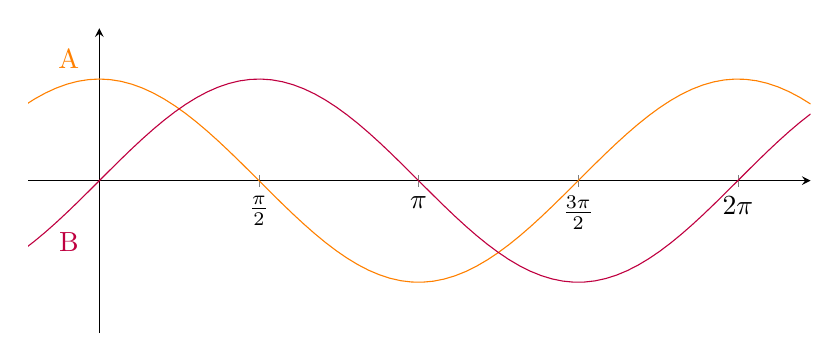
\begin{tikzpicture}
	\begin{axis}[
		axis lines=middle,
		unit vector ratio*=1 1,
		scale=1.45,
		ymin=-1.5, ymax=1.5, xmin=-0.7, xmax=7,
		domain=-3.5:7,
		samples=100,
		ymajorticks=false,
		xtick={ 0.5*pi, pi, 1.5*pi, 2*pi},
		xticklabels={$\frac{\pi}{2}$, $\pi$, $\frac{3\pi}{2}$, $2\pi$},
		disabledatascaling
	]
	\addplot [mark=none, orange] {sin(deg(x+0.5*pi))};
	\node[orange] at (-0.3,1.2) {A};
	
	\addplot [mark=none, purple] {sin(deg(x))};
	\node[purple] at (-0.3,-0.6) {B};
\end{axis}
\end{tikzpicture}\end{center}

\noindent
Przyjrzyjmy się możliwej konstrukcji silnika zasilanego dwufazowo z dwoma biegunami (złożonego z mogącego obracać się magnesu trwałego i dwóch cewek podłączonych po jednej do każdej z faz – cewki tworzą elektromagnesy przyciągające bądź odpychające obracający się magnes trwały):

\begin{center} \begin{tabular}{c|c|c|c|c|c|c|c}
	$t=0$ & &
	$t=\frac{\pi}{2}$ & &
	$t=\pi$ & &
	$t=\frac{3\pi}{2}$ &\\
	\twoPhase{blue}{gray}{90}  & \twoPhase{blue!30}{blue!30}{45} &
	\twoPhase{gray}{blue}{0}   & \twoPhase{red!30}{blue!30}{-45} &
	\twoPhase{red}{gray}{-90}  & \twoPhase{red!30}{red!30}{-135} &
	\twoPhase{gray}{red}{-180} & \twoPhase{blue!30}{red!30}{-225}
\end{tabular} \end{center}

Warto tutaj zauważyć że tak zbudowany silnik jest dość niesymetryczny i dodatkowo może mieć problemy ze startem z pewnych pozycji.
Dlatego w praktyce w takim silniku zastosowano by 4 bieguny (cewki) poprzez dodanie biegunów A' i B' mających działanie odwrotne do A i B (co jest łatwo uzyskać nawijając cewkę „w drugą stronę”):

\begin{center} \begin{tabular}{c|c|c|c|c|c|c|c}
	$t=0$ & &
	$t=\frac{\pi}{2}$ & &
	$t=\pi$ & &
	$t=\frac{3\pi}{2}$ &\\
	\fourPhase{blue}{gray}{red}{gray}{90}  & \fourPhase{blue!30}{blue!30}{red!30}{red!30}{45} &
	\fourPhase{gray}{blue}{gray}{red}{0}   & \fourPhase{red!30}{blue!30}{blue!30}{red!30}{-45} &
	\fourPhase{red}{gray}{blue}{gray}{-90}  & \fourPhase{red!30}{red!30}{blue!30}{blue!30}{-135} &
	\fourPhase{gray}{red}{gray}{blue}{-180} & \fourPhase{blue!30}{red!30}{red!30}{blue!30}{-225}
\end{tabular} \end{center}

Warto jednak zauważyć iż uzyskaliśmy w ten sposób układ 4 fazowy:

\begin{center} 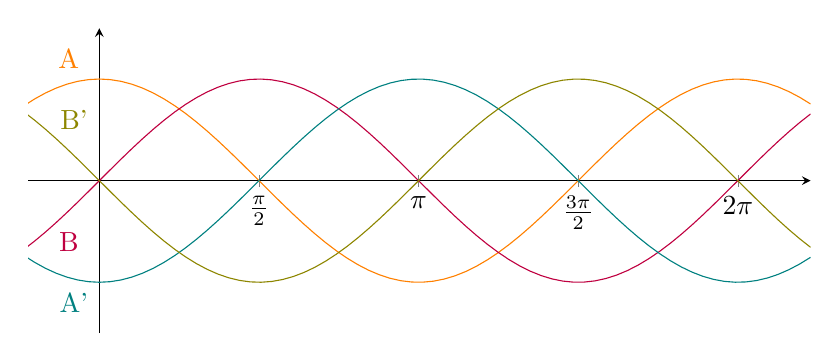
\begin{tikzpicture}
	\begin{axis}[
		axis lines=middle,
		unit vector ratio*=1 1,
		scale=1.45,
		ymin=-1.5, ymax=1.5, xmin=-0.7, xmax=7,
		domain=-3.5:7,
		samples=100,
		ymajorticks=false,
		xtick={ 0.5*pi, pi, 1.5*pi, 2*pi},
		xticklabels={$\frac{\pi}{2}$, $\pi$, $\frac{3\pi}{2}$, $2\pi$},
		disabledatascaling
	]
	\addplot [mark=none, orange] {sin(deg(x+0.5*pi))};
	\node[orange] at (-0.3,1.2) {A};
	
	\addplot [mark=none, purple] {sin(deg(x))};
	\node[purple] at (-0.3,-0.6) {B};
	
	\addplot [mark=none, teal] {sin(deg(x+1.5*pi))};
	\node[teal] at (-0.25,-1.2) {A'};
	
	\addplot [mark=none, olive] {sin(deg(x+pi))};
	\node[olive] at (-0.25,0.6) {B'};
\end{axis}
\end{tikzpicture}\end{center}

Układ dwufazowy był historycznie stosowany z okablowaniem 4 żyłowym (ze względu na brak równoważenia prądu w przewodzie neutralnym).
Został jednak całkowicie wyparty przez układ trójfazowy.

\subsection{podzielona faza}

Układ \href{https://en.wikipedia.org/wiki/Split-phase_electric_power}{podzielonej fazy} można uzyskać stosując transformator z pojedynczym uzwojeniem pierwotnym i podzielonym uzwojeniem wtórnym:

\begin{center} \begin{adjustbox}{scale=0.75} \begin{tikzpicture}
	\begin{scope}[xshift=-1cm]\begin{axis}[
		scale=0.7,
		ymin=-1.5, ymax=1.5, xmin=0, xmax=2*pi,
		domain=0:2*pi,
		samples=100,
		ymajorticks=false,
		xmajorticks=false,
		axis line style={draw=none},
	]
		\addplot [mark=none] {sin(deg(x))};
	\end{axis}\end{scope}

	\begin{scope}[xshift=4cm]
		% primary
		\draw(0, 0)  to [short, o-] +(1, 0)
			to [inductor, bipoles/americaninductor/width=2, bipoles/americaninductor/coils=10]  +(0, 3.5)
			to [short, -o] +(-1, 0);

		% core
		\draw[thick] (1.33, 0.5) -- (1.33, 3);
		\draw[thick] (1.53, 0.5) -- (1.53, 3);

		%secondary
		\draw(3, 0)  to [short, o-] +(-1, 0)
			to [inductor]  +(0, 1.75)
			to [inductor]  +(0, 1.75)
			to [short, -o] +(1, 0);
		\draw(2,1.75) to [short, *-] +(1, 0);
	\end{scope}

	\begin{scope}[xshift=7cm, yshift=.35cm]\begin{axis}[
		scale=0.5,
		ymin=-3, ymax=3, xmin=0, xmax=2*pi,
		domain=0:2*pi,
		samples=100,
		ymajorticks=false,
		xmajorticks=false,
		axis line style={draw=none},
	]
		\addplot [orange, mark=none] {-1.5+sin(deg(x+pi))};
		\addplot [purple, mark=none] { 1.5+sin(deg(x))};
	\end{axis}\end{scope}
\end{tikzpicture} \end{adjustbox} \end{center}

\begin{center} 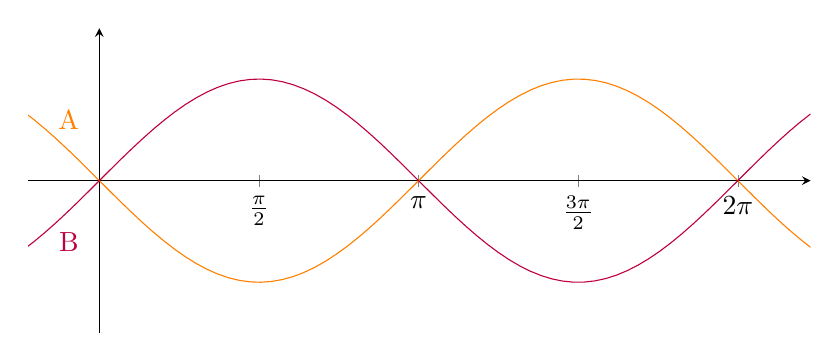
\begin{tikzpicture}
	\begin{axis}[
		axis lines=middle,
		unit vector ratio*=1 1,
		scale=1.45,
		ymin=-1.5, ymax=1.5, xmin=-0.7, xmax=7,
		domain=-3.5:7,
		samples=100,
		ymajorticks=false,
		xtick={ 0.5*pi, pi, 1.5*pi, 2*pi},
		xticklabels={$\frac{\pi}{2}$, $\pi$, $\frac{3\pi}{2}$, $2\pi$},
		disabledatascaling
	]
	\addplot [mark=none, orange] {sin(deg(x+pi))};
	\node[orange] at (-0.3,0.6) {A};
	
	\addplot [mark=none, purple] {sin(deg(x))};
	\node[purple] at (-0.3,-0.6) {B};
\end{axis}
\end{tikzpicture}\end{center}

\noindent
W układzie takim nie jest możliwe użycie silnika wielofazowego:
\begin{center} \begin{tabular}{c|c|c|c|c|c|c|c}
	$t=0$ &
	$t=\frac{\pi}{2}$ &
	$t=\pi$ &
	$t=\frac{3\pi}{2}$\\
	\twoPhase{gray}{gray}{0} &
	\twoPhase{blue}{red}{90} &
	\twoPhase{gray}{gray}{90} &
	\twoPhase{red}{blue}{0}
\end{tabular} \end{center}

\noindent
Uzyskaliśmy co najwyżej oscylacje pomiędzy pozycją $t=\frac{\pi}{2}$ i $t=\frac{3\pi}{2}$.
Jeżeli zastosowalibyśmy cewki w „przeciw fazie” to też nie uzyskamy poprawy:

\begin{center} \begin{tabular}{c|c|c|c|c|c|c|c}
	$t=0$ &
	$t=\frac{\pi}{2}$ &
	$t=\pi$ &
	$t=\frac{3\pi}{2}$\\
	\fourPhase{gray}{gray}{gray}{gray}{-45} &
	\fourPhase{blue}{red}{red}{blue}{135} &
	\fourPhase{gray}{gray}{gray}{gray}{135} &
	\fourPhase{red}{blue}{blue}{red}{-45}
\end{tabular} \end{center}

\noindent
Dzieje się tak dlatego że A' = B oraz B' = A, czyli nie uzyskaliśmy niczego nowego tym zabiegiem.
Wynika to z faktu iż zasada działania tych dodatkowych biegunów silnika jest analogiczna do podzielonej fazy\footnote{
	Można powiedzieć że poprzednio stosując zabieg z użyciem odwrotnie nawiniętych cewek uzyskaliśmy podział faz A i B na połowy, co dało nam układ 4 fazowy.
}, ale podzielonej fazy nie możemy już bardziej podzielić – w wyniku podziału dostaniemy takie same przesunięcia co w wyniku pierwszego podziału.

Podzielona faza może zostać uzyskana także w układzie trójfazowym typu \href{https://en.wikipedia.org/wiki/High-leg_delta}{\textit{High-leg delta}}:

\begin{center} \begin{adjustbox}{scale=1.2} \begin{tikzpicture}
\draw (0,0) to (0,-1.7) node[ground]{};
\draw (0,0) to [inductor, align=left, l=\hspace{-5pt}\color{blue}\scriptsize$U_{AN}\eq$120~V]  (-2.0, 0)
      to [inductor, bipoles/americaninductor/width=1.6, bipoles/americaninductor/coils=8, l=\color{red}\scriptsize$U_{AC}\eq240$~V] (0, 3.0)
      to [inductor, bipoles/americaninductor/width=1.6, bipoles/americaninductor/coils=8, l=\color{red}\scriptsize$U_{BC}\eq240$~V] (2.0, 0)
      to [inductor, align=left, l=\color{blue}\scriptsize$U_{BN}\eq$120~V] (0, 0);
\draw(0,-1.3) to [short, *-o] +(1, 0) node[anchor=west]{N};
\draw(-2.0,0) to [short, *-o] +(-1,0) node[anchor=east]{A};
\draw(2.0, 0) to [short, *-o] +(1, 0) node[anchor=west]{B};
\draw(0, 3)   to [short, *-o] +(0, .7) node[anchor=south]{C};

\draw[red,<->] (-1.8,0.2) -- node[yshift=6pt] {\scriptsize$U_{AB}\eq$240~V} (1.8,0.2);
\draw[orange,<->] (0,0.05) -- node[rotate=90, yshift=6pt] {\scriptsize$U_{CN}\eq$208~V} (0, 2.9);
\end{tikzpicture} \end{adjustbox} \end{center}

Warto zauważyć, iż w układzie podzielonej fazy napięcie międzyfazowe jest zwykłą sumą napięć fazowych. W pokazanym przykładzie: $$U_{AB_{sk}} = 240{\rm ~V} = U_{AN_{sk}} + U_{BN_{sk}} = 120{\rm ~V} + 120{\rm ~V}$$

Układ ten jest powszechnie stosowany w Ameryce Północnej.
Trochę więcej na jego temat (oraz na temat instalacji elektrycznych w USA) można dowiedzieć się z: \url{https://www.youtube.com/watch?v=fJeRabV5hNU}.

\subsection{trzy fazy}

Najpowszechniej stosowanym system wytwarzania i dystrybucji energii elektrycznej jest \href{https://en.wikipedia.org/wiki/Three-phase_electric_power}{układ trójfazowy}, w którym przesunięcie pomiędzy kolejnymi fazami wynosi $\frac{2\pi}{3}$.

\newcommand{\threesixPhase}[7] {
	\begin{adjustbox}{scale=0.43}
	\begin{tikzpicture}
		\tikzstyle{fullrotate}=[rotate=##1,nodes={rotate=##1}]
		\tikzstyle{coil}=[align=center, minimum height=0.7cm, minimum width=0.7cm, fill=##1]
		
		\node[coil=#1] at (0,1.7) {A};
		\begin{scope}[fullrotate=-120]
			\node[coil=#2] at (0,1.7) {B};
		\end{scope}
		\begin{scope}[fullrotate=120]
			\node[coil=#3] at (0,1.7) {C};
		\end{scope}
		
		\begin{scope}[fullrotate=180]
			\node[coil=#4] at (0,1.7) {\aprim};
		\end{scope}
		\begin{scope}[fullrotate=60]
			\node[coil=#5] at (0,1.7) {\bprim};
		\end{scope}
		\begin{scope}[fullrotate=-60]
			\node[coil=#6] at (0,1.7) {\cprim};
		\end{scope}
		
		\node[coil=none] at (0,1.9) {};
		
		\begin{scope}[fullrotate=#7]
			\fill[blue] (-1,-0.35) rectangle (0,0.35);
			\node at (-0.5,0) {N};
			\fill[red] (0,-0.35) rectangle (1,0.35);
			\node at (0.5,0) {S};
		\end{scope}
	\end{tikzpicture}
	\end{adjustbox}
}
\newcommand{\threePhase}[4] {
	\def\aprim{}\def\bprim{}\def\cprim{}
	\threesixPhase{#1}{#2}{#3}{none}{none}{none}{#4}
}
\newcommand{\sixPhase}[7] {
	\def\aprim{A'}\def\bprim{B'}\def\cprim{C'}
	\threesixPhase{#1}{#2}{#3}{#4}{#5}{#6}{#7}
}


\begin{center} 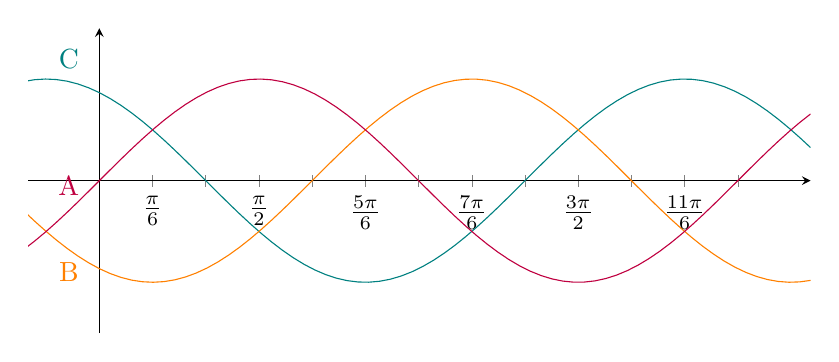
\begin{tikzpicture}
	\begin{axis}[
		axis lines=middle,
		unit vector ratio*=1 1,
		scale=1.45,
		ymin=-1.5, ymax=1.5, xmin=-0.7, xmax=7,
		domain=-3.5:7,
		samples=100,
		ymajorticks=false,
		xtick={pi/6, 2*pi/6, 3*pi/6, 4*pi/6, 5*pi/6, 6*pi/6, 7*pi/6, 8*pi/6, 9*pi/6, 10*pi/6, 11*pi/6, 12*pi/6},
		xticklabels={$\frac{\pi}{6}$, ~, $\frac{\pi}{2}$, ~, $\frac{5\pi}{6}$, ~, $\frac{7\pi}{6}$, ~, $\frac{3\pi}{2}$, ~, $\frac{11\pi}{6}$, ~},
		disabledatascaling
	]
	\addplot [mark=none, teal] {sin(deg(x+2*pi/3))};
	\node[teal] at (-0.3,1.2) {C};
	
	\addplot [mark=none, orange] {sin(deg(x+4*pi/3))};
	\node[orange] at (-0.3,-0.9) {B};
	
	\addplot [mark=none, purple] {sin(deg(x))};
	\node[purple] at (-0.3,-0.05) {A};
\end{axis}
\end{tikzpicture}\end{center}

\noindent
Przyjrzyjmy się możliwej konstrukcji silnika zasilanego trójfazowo:

\begin{center} \begin{tabular}{c|c|c|c|c|c}
	$t=\frac{\pi}{6}$ &
	$t=\frac{\pi}{2}$ &
	$t=\frac{5\pi}{6}$ &
	$t=\frac{7\pi}{6}$ &
	$t=\frac{3\pi}{2}$ &
	$t=\frac{11\pi}{6}$\\
	\threePhase{blue!25}{red}{blue!25}{150} &
	\threePhase{blue}{red!25}{red!25}{90} &
	\threePhase{blue!25}{blue!25}{red}{30} &
	\threePhase{red!25}{blue}{red!25}{-30} &
	\threePhase{red}{blue!25}{blue!25}{-90} &
	\threePhase{red!25}{red!25}{blue}{-150}
\end{tabular} \end{center}
%
Oczywiście tutaj także możemy wprowadzić dodatkowe bieguny A', B' i C' o działaniu przeciwny do A, B i C (poprzez odwrotne nawinięcie ich cewek):
%
\begin{center} \begin{tabular}{c|c|c|c|c|c}
	$t=\frac{\pi}{6}$ &
	$t=\frac{\pi}{2}$ &
	$t=\frac{5\pi}{6}$ &
	$t=\frac{7\pi}{6}$ &
	$t=\frac{3\pi}{2}$ &
	$t=\frac{11\pi}{6}$\\
	\sixPhase{blue!25}{red}{blue!25}{red!25}{blue}{red!25}{150} &
	\sixPhase{blue}{red!25}{red!25}{red}{blue!25}{blue!25}{90} &
	\sixPhase{blue!25}{blue!25}{red}{red!25}{red!25}{blue}{30} &
	\sixPhase{red!25}{blue}{red!25}{blue!25}{red}{blue!25}{-30} &
	\sixPhase{red}{blue!25}{blue!25}{blue}{red!25}{red!25}{-90} &
	\sixPhase{red!25}{red!25}{blue}{blue!25}{blue!25}{red}{-150}
\end{tabular} \end{center}
%
Co daje nam funkcjonalny odpowiednik układu 6cio fazowego o przesunięciu $\frac{\pi}{3}$:
%
\begin{center} 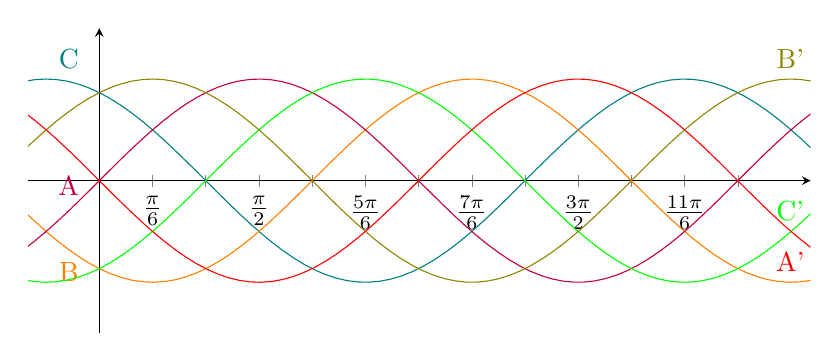
\begin{tikzpicture}
	\begin{axis}[
		axis lines=middle,
		unit vector ratio*=1 1,
		scale=1.45,
		ymin=-1.5, ymax=1.5, xmin=-0.7, xmax=7,
		domain=-3.5:7,
		samples=100,
		ymajorticks=false,
		xtick={pi/6, 2*pi/6, 3*pi/6, 4*pi/6, 5*pi/6, 6*pi/6, 7*pi/6, 8*pi/6, 9*pi/6, 10*pi/6, 11*pi/6, 12*pi/6},
		xticklabels={$\frac{\pi}{6}$, ~, $\frac{\pi}{2}$, ~, $\frac{5\pi}{6}$, ~, $\frac{7\pi}{6}$, ~, $\frac{3\pi}{2}$, ~, $\frac{11\pi}{6}$, ~},
		disabledatascaling
	]
	\addplot [mark=none, teal] {sin(deg(x+2*pi/3))};
	\node[teal] at (-0.3,1.2) {C};
	
	\addplot [mark=none, orange] {sin(deg(x+4*pi/3))};
	\node[orange] at (-0.3,-0.9) {B};
	
	\addplot [mark=none, purple] {sin(deg(x))};
	\node[purple] at (-0.3,-0.05) {A};
	
	
	\addplot [mark=none, green] {sin(deg(x+5*pi/3))};
	\node[green] at (6.8, -0.3) {C'};
	
	\addplot [mark=none, olive] {sin(deg(x+7*pi/3))};
	\node[olive] at (6.8,1.2) {B'};
	
	\addplot [mark=none, red] {sin(deg(x+pi))};
	\node[red] at (6.8,-0.8) {A'};
	
\end{axis}
\end{tikzpicture}\end{center}
%
Warto jednak zauważyć że 3 fazy są najmniejszą liczbą faz, dla których taki zabieg nie jest konieczny.


\subsubsection{napięcie międzyfazowe}

\noindent
Pamiętając że napięcie to różnica potencjałów\footnote{i że napięcie fazowe w postaci sinusoidy, jest różnicą potencjału przewodu fazowego i przewodu neutralnego}, możemy obliczyć napięcie między fazowe:
	$$U_{AN} = V_A - V_N \qquad U_{BN} = V_B - V_N \qquad U_{AB} = V_A - V_B$$
	$$U_{AB} = (U_{AN} + V_N) - (U_{BN} + V_N) = U_{AN} - U_{BN}$$
Jak widzimy jest ono różnicą napięć fazowych (a nie ich sumą).
Należy jednak mieć na uwadze że jest to różnica przesuniętych w fazie sinusoid (a nie stałych wartości i z tego powodu napięcie to nie wynosi zero):
	$$U_{AB} = U_{AN} - U_{BN} = U_0 \cdot \sin(t) - U_0 \cdot \sin\left( t + \frac{2\pi}{3} \right)$$
	$$U_{AB} = U_0 \left( \sin(t) - \sin\left( t + \frac{2\pi}{3} \right) \right)$$
gdzie $U_0$ to amplituda napięcia fazowego.
%
Korzystając z tożsamości trygonometrycznej: $\sin(x) - \sin(y) = 2 \cdot \sin(\frac{x - y}{2}) \cdot \cos(\frac{x + y}{2})$ otrzymujemy:
	$$U_{AB} = U_0 \cdot 2 \cdot \sin\left( \frac{t - (t + \frac{2\pi}{3})}{2} \right) \cdot \cos\left( \frac{t + (t + \frac{2\pi}{3})}{2} \right)$$
	$$U_{AB} = U_0 \cdot 2 \cdot \sin\left( -\frac{\pi}{3} \right) \cdot \cos\left( t + \frac{\pi}{3} \right) = U_0 \cdot 2 \cdot \frac{\sqrt{3}}{2} \cdot \cos\left( t + \frac{\pi}{3} \right)$$
	$$U_{AB} = \sqrt{3} \cdot U_0 \cdot \cos\left( t + \frac{\pi}{3} \right)$$
Obliczenia dla pozostałych napięć międzyfazowych są analogiczne.
Widzimy zatem że napięcie międzyfazowe będzie przesunięte względem napięć rozważanych faz i będzie miało amplitudę (a zatem także wartość międzyszczytową i skuteczną) $\sqrt{3}$ raza większą od wartości napięcia fazowego.

\begin{center} \begin{adjustbox}{scale=0.75} \begin{tikzpicture}
	\begin{axis}[
		axis lines=middle,
		unit vector ratio*=1 1,
		scale=2.5,
		ymin=-2.2, ymax=2.2, xmin=-3.2, xmax=7,
		domain=-3.5:7,
		samples=100,
		ytick={ -sqrt(3), -1, 1, sqrt(3)},
		yticklabels={$-\sqrt{3} \cdot U_0$, $-U_0$, $U_0$, $\sqrt{3} \cdot U_0$},
		xtick={ 0.5*pi, pi, 1.5*pi, 2*pi},
		xticklabels={$\frac{\pi}{2}$, $\pi$, $\frac{3\pi}{2}$, $2\pi$},
		disabledatascaling
	]
	\addplot [mark=none, orange] {sin(deg(x+2*pi/3))};
	\node[orange] at (-1.9,0.45) {A};
	
	\addplot [mark=none, purple] {sin(deg(x))};
	\node[purple] at (-1.9,-0.75) {B};
	
	\addplot [mark=none, blue] {sin(deg(x+2*pi/3)) - sin(deg(x))};
	\node[blue] at (-2.02,1.4) {A-B};
	
	%\addplot [mark=none, red] {sqrt(3) * cos(deg(x+pi/3))};
	%\node[red] at (-2.02,1.4) {A-B};
\end{axis}
\end{tikzpicture} \end{adjustbox} \end{center}


\subsubsection{trójkąt-gwiazda}

Istnieją i są stosowane dwa sposoby połączeń uzwojeń (zarówno silników, generatorów, jak i transformatorów) w systemach trójfazowych - trójkąt (delta $\Delta$) i gwiazda (star, Y).
Przy połączeniu w trójkąt nie dostajemy (przy generatorze, uzwojeniu wtórnym transformatora) / nie używamy (przy silnikach) przewodu neutralnego – operujemy tylko na napięciach międzyfazowych.
W przypadku połączenia w gwiazdę możemy (ale nie musimy) korzystać z punktu neutralnego.

Typowo transformatory energetyczne z średniego na niskie napięcie działają w układzie trójkąt-gwiazda, czyli po stronie pierwotnej (średniego napięcia) uzwojenia łączone są w trójką, a po stronie wtórnej (400V) w gwiazdę.
Dzięki temu dostępny jest po stronie wtórnej punkt neutralny i możliwe jest korzystanie zarówno z napięć międzyfazowych (400V) jak i jednofazowych L-N (230V).

\begin{center} \begin{adjustbox}{scale=1.0} \begin{tikzpicture}

	\begin{scope}[xshift=-4cm,yshift=-1.7cm]
		\ctikzset{bipoles/americaninductor/width=1.6, bipoles/americaninductor/coils=8}
		\draw (-2.0,0) to [inductor] (2.0, 0) to [inductor] (0, 3.0) to [inductor] (-2.0,0);
		\draw(-2.0,0) to [short, *-o] +(-1,0) node[anchor=east]{A};
		\draw(2.0, 0) to [short, *-o] +(1, 0) node[anchor=west]{B};
		\draw(0, 3)   to [short, *-o] +(0, .7) node[anchor=south]{C};
		
		\draw[red,<->] (-2.0,-0.2) -- node[below] {\scriptsize$U_{AB}\eq$400~V} (2.0,-0.2);
		\draw[red,<->] (-2.15,0.15) -- node[above, sloped] {\scriptsize$U_{AC}\eq$400~V} (-0.22,3);
		\draw[red,<->] (2.15,0.15) -- node[above, sloped] {\scriptsize$U_{BC}\eq$400~V} (0.22,3);
		
		\node at (0,-1.3) {\bf trójkąt (delta, $\Delta$)};
	\end{scope}

	\begin{scope}[xshift=4cm]
		\draw (0,0) to [inductor] (-1.3, -1.3) to [short, -o] +(-0.9,0) node[anchor=east]{A};
		\draw (1.3, -1.3) to [inductor] (0,0); \draw (1.3, -1.3) to [short, -o] +(0.9, 0) node[anchor=west]{B};
		\draw (0,0) to [inductor] (0, 1.8) to [short, -o] +(0, 0.3) node[anchor=south]{C};
		\draw(0,0) to [short, *-o] +(0, -2.0) node[anchor=north]{N};
		
		\draw[red,<->] (-2.3,-1.7) -- node[above] {\scriptsize$U_{AB}\eq$400~V} (2.3,-1.7);
		\draw[red,<->] (-2.25,-1.05) -- node[above, sloped] {\scriptsize$U_{AC}\eq$400~V} (-0.22,2.1);
		\draw[red,<->] (2.25,-1.05) -- node[above, sloped] {\scriptsize$U_{BC}\eq$400~V} (0.22,2.1);
		
		\draw[blue,<->] (-1.35,-1.05) -- node[above, sloped] {\scriptsize$U_{AN}\eq$230~V} (-0.35, -0.05);
		\draw[blue,<->] (1.35,-1.05) -- node[above, sloped] {\scriptsize$U_{BN}\eq$230~V} (0.35, -0.05);
		\draw[blue,<->] (0.15,0.05) -- node[below, sloped, align=left, font=\scriptsize] {~$U_{CN}\eq$\\~230~V} (0.15, 1.7);
		
		\node at (0,-3) {\bf gwiazda (star, Y)};
	\end{scope}
\end{tikzpicture} \end{adjustbox} \end{center}
%
Należy zauważyć że podłączenie uzwojeń (o takiej samej impedancji) w gwiazdę skutkuje mniejszym poborem prądu niż podłączenie ich w trójkąt.
Jest to efektem tego że w połączeniu typu gwiazda napięcia na poszczególnych uzwojeniach są mniejsze ($\sqrt{3}$ raza) niż w przypadku połączenia w trójkąt (230V vs 400V).

% Copyright (c) 2021 Robert Ryszard Paciorek <rrp@opcode.eu.org>
% 
% MIT License
% 
% Permission is hereby granted, free of charge, to any person obtaining a copy
% of this software and associated documentation files (the "Software"), to deal
% in the Software without restriction, including without limitation the rights
% to use, copy, modify, merge, publish, distribute, sublicense, and/or sell
% copies of the Software, and to permit persons to whom the Software is
% furnished to do so, subject to the following conditions:
% 
% The above copyright notice and this permission notice shall be included in all
% copies or substantial portions of the Software.
% 
% THE SOFTWARE IS PROVIDED "AS IS", WITHOUT WARRANTY OF ANY KIND, EXPRESS OR
% IMPLIED, INCLUDING BUT NOT LIMITED TO THE WARRANTIES OF MERCHANTABILITY,
% FITNESS FOR A PARTICULAR PURPOSE AND NONINFRINGEMENT. IN NO EVENT SHALL THE
% AUTHORS OR COPYRIGHT HOLDERS BE LIABLE FOR ANY CLAIM, DAMAGES OR OTHER
% LIABILITY, WHETHER IN AN ACTION OF CONTRACT, TORT OR OTHERWISE, ARISING FROM,
% OUT OF OR IN CONNECTION WITH THE SOFTWARE OR THE USE OR OTHER DEALINGS IN THE
% SOFTWARE.

\section{Silniki}

Silnik jest urządzeniem do zamiany energii elektrycznej na energię mechaniczną (prawie zawsze) ruchu obrotowego (który potem może być zamieniany na inne postaci ruchu).
W konstrukcji mechanicznej silnika wyróżnia się:
\begin{itemize}
	\item \strong{wirnik} – element obracający się
	\item \strong{stojan} – element pozostający nieruchomo wewnątrz którego obraca się wirnik
\end{itemize}

Możliwe konstrukcje silników wielofazowych rozważaliśmy już przy omawianiu zagadnienia prądu wielofazowego, w oparciu o obracanie magnesu trwałego przy pomocy układu cewek zasilanych z poszczególnych faz.
Pośrednio (przy rozważaniu układu podzielonej fazy) przyjrzeliśmy się nawet możliwości konstrukcji silnika jednofazowego – nie udało nam się.
Model ten dość dobrze oddaje koncepcję budowy rzeczywistych silników elektrycznych.
I w każdym typie silnika konieczne jest zapewnienie co najmniej dwóch faz, aby móc uzyskać wirujące (a nie tylko zmienne – jak przy jednej fazie) pole magnetyczne.

Dlatego też najprostszym koncepcyjnie silnikiem jest silnik trójfazowy prądu przemiennego z magnesami stałymi w wirniku i elektromagnesami w stojanie, czyli właśnie taki jak rozważaliśmy przy prądzie trójfazowym.
Zamiast magnesów trwałych na wirniku mogą być umieszczone elektromagnesy zasilane prądem stałym (doprowadzonym poprzez szczotki).
Silniki tego typu określa się mianem \strong{silników synchronicznych} gdyż ich prędkość obrotowa jest równa prędkości wirowania pola magnetycznego.

Wadą takich silników jest trudność w ich rozruchu – taki silnik (podłączony bezpośrednio do sieci elektrycznej) nie zacznie się obracać.
Spowodowane to jest tym iż pole magnetyczne w stojanie będzie zmieniało się zbyt szybko, aby pokonać bezwładność mechaniczną wirnika i wprawić go w ruch.

Stosowane jest kilka mechanizmów na rozruch takiego silnika (np. rozruch jako silnika asynchronicznego, co wyklucza stosowanie magnesów trwałych na wirniku).
Współcześnie do rozruchu tego typu silników wykorzystywane są elektroniczne przemienniki częstotliwości (falowniki),
	które pozwalają na uruchomienie takiego silnika przy wolno zmiennym polu magnetycznym stojana, jak również na płynne sterowanie prędkością obrotową silnika.

\subsection{silniki indukcyjne (asynchroniczne AC)}

Główna różnica w stosunku co do silnika synchronicznego polega na wykonaniu wirnika – znajdują się na nim uzwojenia w których (za sprawą zmiennego pola magnetycznego stojana) indukowany jest prąd (dlatego \textit{silnik indukcyjny}).
Jego przepływ powoduje powstanie pola magnetycznego wirnika (przekształcenie wirnika w magnes), dzięki czemu zaczyna się obracać.
Aby proces indukcji mógł zachodzić wirnik musi obracać się wolniej niż wirowanie pola magnetycznego stojana (czyli wolniej niż wynikałoby z częstotliwości zasilania, dlatego \textit{silnik asynchroniczny}).
Wirnik często wykonywany jest w postaci klatki (stanowiącej od razu jego uzwojenie), dlatego większość silników tego typu to \strong{silniki klatkowe}.

\noindent Więcej informacji: \url{https://www.youtube.com/watch?v=59HBoIXzX_c}

\subsection{silniki jednofazowe AC}

Jak się przekonaliśmy silnik z jedną fazą nie działa – jedna faza daje zmienne pole, ale one nie rotuje (nie determinuje kierunku obrotu, nie powoduje rozpoczęcia obrotu).
Dlatego w silnikach jednofazowych prądu przemiennego wytwarzana jest druga faza z użyciem kondensatora (który jak wiemy wprowadza przesunięcie fazowe prądu).
Koncepcyjnie są to silniki takie jak omawiane przy prądzie dwufazowym, wykonywane najczęściej jako asynchroniczne (klatkowe).

\noindent Więcej informacji: \url{https://www.youtube.com/watch?v=jNWlWzFzHi4}

\subsection{silniki prądu stałego (DC)}

W klasycznym silniku prądu stałego wirowanie pola magnetycznego uzyskuje się poprzez komutację mechaniczną.
W rozwiązaniu takim w stojanie znajdują się magnesy trwałe, a na wirniku uzwojenia.
Komutator zmienia biegunowość uzwojeń wirnik tak aby obracał się on względem stojana.

\noindent Więcej informacji: \url{https://www.youtube.com/watch?v=GQatiB-JHdI}

\subsection{bezszczotkowe silniki prądu stałego (BLDC)}

W silniku BLDC mamy nieruchome elektromagnesy (w stojanie) i magnes trwały na wirniku (czyli tak jak w silniku synchronicznym z magnesami trwałymi).
Sterownik silnika, będący elektroniczną formą komutatora, zasila kolejno cewki poszczególnych „faz” co powoduje ruch wirnika przyciąganego/odpychanego przez odpowiednie elektromagnesy (analogicznie jak w wspomnianym silnku AC).
Główna różnica polega na napięciu zasilania oraz kształcie sygnałów podawanych na cewki – w silniku BLDC będzie on na ogół przypominał prostokąt a nie sinus.

\subsection{silniki krokowe}

Sa to silniki bardzo zbliżone do BLDC – również mamy elektromagnesy w stojanie i magnesy trwałe na wirniku.
Główna różnica polega w zastosowaniu i sposobie sterowania.
Sterując BLDC zależy nam na prędkości obrotowej, a sterując silnikiem krokowym zależy nam na wykonaniu określonej liczby kroków.
Często będą występować też różnice konstrukcyjne – w ilości faz, cewek w stojanie, biegunów na wirniku, itd.
W silnikach krokowych z każdą fazą działania silnika następuje tylko niewielkie (często stanowiące niewielki ułamek pełnego obrotu) obrócenie wirnika.
Z każdym impulsem sterującym silnik wykonuje taki jeden krok.
Sposób wysterowania sprawia także że silnik taki ma duży moment trzymający (kosztem energochłonności).

\noindent Więcej informacji: \url{https://www.youtube.com/watch?v=09Mpkjcr0bo}

\subsection{podsumowanie}

Warto zauważyć upowszechnianie się elektronicznych systemów sterowania silnikami.
Falowniki pozwalają na łatwe stosowanie silików trójfazowych w obwodach jednofazowych oraz pozwalają także na stosowanie silników synchronicznych z magnesami trwałymi, łatwe kontrolowanie prędkości obrotowej silników AC.
Należy jednak zwrócić uwagę na podobieństwa w działaniu przestawionych typów silników elektrycznych (np. BLDC do synchronicznego AC z magnesami stałymi sterowanego przez falownik).

W przedstawionych tutaj opisach zostały prawie całkowicie pominięte zagadnienia związane z mechaniczną konstrukcją silników,
	a także rozwiązaniami takimi jak np. umieszczenie więcej niż dwóch biegunów na wirniku (np. 4 w kolejności NSNS), co oczywiście wpływa też na układ elektromagnesów zasilanych z poszczególnych faz.

% Copyright (c) 2011-2021 Robert Ryszard Paciorek <rrp@opcode.eu.org>
% 
% MIT License
% 
% Permission is hereby granted, free of charge, to any person obtaining a copy
% of this software and associated documentation files (the "Software"), to deal
% in the Software without restriction, including without limitation the rights
% to use, copy, modify, merge, publish, distribute, sublicense, and/or sell
% copies of the Software, and to permit persons to whom the Software is
% furnished to do so, subject to the following conditions:
% 
% The above copyright notice and this permission notice shall be included in all
% copies or substantial portions of the Software.
% 
% THE SOFTWARE IS PROVIDED "AS IS", WITHOUT WARRANTY OF ANY KIND, EXPRESS OR
% IMPLIED, INCLUDING BUT NOT LIMITED TO THE WARRANTIES OF MERCHANTABILITY,
% FITNESS FOR A PARTICULAR PURPOSE AND NONINFRINGEMENT. IN NO EVENT SHALL THE
% AUTHORS OR COPYRIGHT HOLDERS BE LIABLE FOR ANY CLAIM, DAMAGES OR OTHER
% LIABILITY, WHETHER IN AN ACTION OF CONTRACT, TORT OR OTHERWISE, ARISING FROM,
% OUT OF OR IN CONNECTION WITH THE SOFTWARE OR THE USE OR OTHER DEALINGS IN THE
% SOFTWARE.

\section{Układy zasilania}

\subsection{Związek z potencjałem ziemi (układy sieci - IT, TT, TN)}

Wyróżnia się kilka \href{https://en.wikipedia.org/wiki/Earthing_system}{układów sieci zasilającej}. Poszczególne układy posiadają kilku literowe oznaczenia w których:
\begin{itemize}
	\item pierwsza litera (\strong{I} lub \strong{T}) oznacza relację punktu neutralnego transformatora i potencjału ziemi:
	\begin{itemize}
		\item \strong{I} – punkt neutralny transformatora izolowany od ziemi (lub połączony poprzez dużą impedancję)
		\begin{itemize}
			\item uzwojenie wtórne transformatora może nie posiadać punktu neutralnego (np. może być połączone w trójkąt)
			\item przewód neutralny nie musi (ale może) występować w instalacji
			\item nie da się odróżnić przewodu neutralnego od pojedynczego przewodu fazowego – w obu wypadkach potencjał względem ziemi jest nieustalony
			\item znaczenie mają jedynie napięcia pomiędzy przewodami fazowymi oraz fazowymi i neutralnym (jeżeli występuje)
		\end{itemize}
		\item \strong{T} – punkt neutralny transformatora połączony z ziemią
		\begin{itemize}
			\item uzwojenie wtórne transformatora musi posiadać punkt neutralny (typowo jest uzwojeniem typu gwiazda)
			\item przewód neutralny ma potencjał równy potencjałowi ziemi, zatem inne napięcia odnoszą się także do potencjału ziemi (np. w przewodzie fazowym jest 230V względem Ziemi)
		\end{itemize}
	\end{itemize}
	\item druga litera (\strong{T} lub \strong{N}) oznacza sposób połączenia części normalnie nieprzewodzących z potencjałem ziemi:
		\item \strong{T} – połączenie za pomocą lokalnego uziomu lub uziomu grupowego (obejmującego kilka odbiorników) nie połączonego z uziomem punktu neutralnego transformatora
		\item \strong{N} – połączenie poprzez uziom punktu neutralnego transformatora, w tym wypadku występują kolejne oznaczenia informujące w jaki sposób realizowane jest to połączenie:
		\begin{itemize}
			\item \strong{S} - przy pomocy osobnego przewodu ochronnego PE dochodzącego do stacji transformatorowej
			\item \strong{C} - przy pomocy wspólnego przewodu ochronnego i neutralnego PEN\footnote{\label{PEN}Przewód PEN powinien mieć przekrój minimum 10mm$^2$ Cu lub 16mm$^2$ Al}$^,$\footnote{Układ nie jest dopuszczony do stosowania w budynkach na terenie Polski.}
			\item \strong{C-S} - na części trasy (od stacji transformatorowej do punktu rozdziału PEN\footnoteref{PEN}, np. w złączu lub rozdzielni głównej\footnote{Punkt taki powinien być uziemiony.})
			w postaci wspólnego przewodu ochronnego i neutralnego PEN, dalej w postaci osobnego przewodu ochronnego PE
		\end{itemize}
\end{itemize}
%
Wyróżnia się układy:
\begin{itemize}
	\item \strong{IT} – punkt neutralny transformatora izlowoany lub nie wystepuje, uziemienia urządzeń łączone lokalnie do ziemi
	\item \strong{TT} – punkt neutralny transformatora połączony z ziemią, uziemienia urządzeń łączone lokalnie do ziemi
	\item \strong{TN} – punkt neutralny transformatora połączony z ziemią, uziemienia urządzeń łączone do uziemienia punktu neutralnego transformatora, przy pomocy:
	\begin{itemize}
		\item przewodu PE  – układ \strong{TN-S}
		\item przewodu PEN – układ \strong{TN-C}
		\item przewodu PEN (bliżej transformatora) i PE (bliżej odbiornika) – układ \strong{TN-C-S}
	\end{itemize}
\end{itemize}

\subsubsection{układ IT}
\begin{itemize}
	\item Dzięki izolowaniu wszystkich przewodów roboczych od potencjału ziemi pierwsze zwarcie doziemne\footnote{bez względu na to czy przewodu fazowego czy neutralnego} w tym układzie związane jest z przepływem niskiego prądu zwarciowego.
	\begin{itemize}
		\item Wartość prądu takiego zwarcia zależy od wielkości sieci (wielkości pojemności sieć-ziemia) i często jest rzędu kilku mA, czyli może nie spowodować nawet zadziałania RCD.
		\item Napięcie które po takim zwarciu będzie występować pomiędzy pozostałymi przewodami a ziemią zależy od tego czy zwarciu uległ przewód neutralny czy fazowy
			(bo ziemia zaczyna pełnić jego funkcje, czyli możemy mieć np. napięcie międzyfazowe między ziemią a dowolną z nie zwartych faz).
		\item Można powiedzieć że w momencie wystąpienia pierwszego zwarcia doziemnego układ przechodzi w układ TT (przy czym impedancja uziemienia "punktu neutralnego", powstała na skutek zwarcia, jest nieznanej jakości).
	\end{itemize}
	\item Układ może być (i często jest) stosowany:
	\begin{itemize}
		\item w celu zwiększenia niezawodności (np. na salach operacyjnych) - pierwsze zwarcie jest sygnalizowane, ale nie powoduje wyłączenia; układ uzyskiwany z lokalnego trafo separacyjnego 1:1 zasilanego z „normalnej” sieci TN
		\item w celu zwiększenia bezpieczeństwa (przeciw iskrzeniu, np. w kopalniach) - prąd pierwszego zwarcia jest niewielki, więc zmniejsza ryzyko powstania iskry; pierwsze zwarcie powoduje automatyczne wyłączenie obwodu
		\item w przypadkach gdzie „trudno znaleźć ziemię” w celu uziemienia punktu neutralnego (np. na statkach)
	\end{itemize}
	\item Układ pozwala na rezygnację z przewodu neutralnego (i stosowanie wyłącznie napięć międzyfazowych, ale nie jest to wymogiem\footnote{
			Rezygnacja z przewodu neutralnego i stosowanie tylko napięć międzyfazowych eliminuje także problem przerwania przewodu neutralnego skutkującego ryzykiem pojawienia się napięcia międzyfazowego na odbiornikach jednofazowych.
		}.
	\item Układ ten wymaga stosowania zabezpieczeń dwupolowych (dla odbiorów zasilanych faza-neutralny lub faza-faza).
	\item W układzie powinny być stosowane układy sygnalizujące wystąpienie pierwszego zwarcia doziemnego / układy kontroli stanu izolacji.
	\item Główną wadą takiego układu jest gorsza (wyższa) niż w TN (a często także niż w TT) impedancja pętli podwójnego zwarcia doziemnego, co może prowadzić do braku odpowiednio szybkiego wyłączenia takiego zwarcia.
\end{itemize}

\subsection{prąd zwarcia}

\begin{center}\includegraphics{img/elektryka/prad_zwarciowy}\end{center}

Przy projektowaniu instalacji i doborze zabezpieczeń istotna rolę odgrywa prąd zwarcia.
Oblicza się go w oparciu o dane transformatora i parametry linii przesyłowych (grubość i materiał kabli, co przekłada się na ich rezystancję) zgodnie z poniższymi zasadami:

\begin{itemize}
	\item dane do obliczeń – parametry transformatora:
	\begin{itemize}
		\item prąd nominalny $I_n$, czyli prąd uzwojenia wtórego przy nominalnym obciążeniu transformatora
		\item nominalne napięcie strony pierwotnej $U_P$ oraz strony wtórnej $U_n$
		\item napięcie zwarcia $U_k$, czyli napięcie na uzwojeniu pierwotnym powodujące przepływ nominalnego prądu na zwartym uzwojeniu wtórnym,
			typowo podane w postaci $U_k{\rm [\%]}$, czyli wyrażone jako procent nominalnego napięcia uzwojenia pierwotnego:
				$$U_k{\rm [\%]}=\frac{U_p}{U_k}$$
	\end{itemize}
	\item prąd zwarcia $I_{k1}$ na zaciskach transformatora (czyli w w obwodzie zamykanym przez S1) obliczamy w oparciu o parametry T1:
		$$I_{k1} = \frac{I_n}{U_k[\%]}$$
	\item rezystancję wewnętrzną $R_w$ transformatora obliczamy w oparciu o napięcie nominalne strony wtórnej $U_n$ i prąd $I_{k1}$:
		$$R_w = \frac{U_n}{I_{k1}} = \frac{U_n \cdot U_k{\rm [\%]}}{I_n}$$
	\item dzięki temu możemy obliczyć prąd zwarcia instalacji:
		$$I_{k2} = \frac{U_n}{Rw + Ri} = \frac{U_n}{U_n \cdot U_k[\%]/I_n + R_i}$$
\end{itemize}

\noindent\strong{Przykład:}
\begin{itemize}
	\item trafo na 400V ($U_n=400{\rm ~V}$) o mocy 1.2MW ($I_n=1800{\rm ~A}$) i napięciu zwarcia $U_k{\rm [\%]}=6\%$
	\item szyna Cu o przekroju $800{\rm ~mm^2}$ i długości 1m ($R_i = 0.00004545~\Omega$)
	\item zatem $I_{k2} = 400 / (400 \cdot 0.06/1800 + 0.00004545) = 29.898{\rm ~kA}$
\end{itemize}
\vspace{8pt}

Jest to prosty sposób obliczania spodziewanego prądu zwarcia.
Obliczenia w projekcie powinny zawsze uwzględniać wszystkie czynniki i być wykonywane zgodnie z normami.
Autor nie ponosi odpowiedzialności za skutki błędnego zastosowania tego schematu obliczeń.

Po wykonaniu instalacji (oraz okresowo) dokonuje się pomiarów impedancji pętli zwarcia, które mają na celu ustalenie rzeczywistego (minimalnego) prądu zwarcia.
Jest on istotny ze względu na skuteczność zadziałania zabezpieczeń nadprądowych.
Konieczność wykonania pomiarów a nie tylko oparcia się na obliczeniu wynika m.in. z faktu iż mogły pojawić się w instalacji nieprzewidziane rezystancje (np. niedokręcony zacisk śrubowy).

% Copyright (c) 2021 Robert Ryszard Paciorek <rrp@opcode.eu.org>
% 
% MIT License
% 
% Permission is hereby granted, free of charge, to any person obtaining a copy
% of this software and associated documentation files (the "Software"), to deal
% in the Software without restriction, including without limitation the rights
% to use, copy, modify, merge, publish, distribute, sublicense, and/or sell
% copies of the Software, and to permit persons to whom the Software is
% furnished to do so, subject to the following conditions:
% 
% The above copyright notice and this permission notice shall be included in all
% copies or substantial portions of the Software.
% 
% THE SOFTWARE IS PROVIDED "AS IS", WITHOUT WARRANTY OF ANY KIND, EXPRESS OR
% IMPLIED, INCLUDING BUT NOT LIMITED TO THE WARRANTIES OF MERCHANTABILITY,
% FITNESS FOR A PARTICULAR PURPOSE AND NONINFRINGEMENT. IN NO EVENT SHALL THE
% AUTHORS OR COPYRIGHT HOLDERS BE LIABLE FOR ANY CLAIM, DAMAGES OR OTHER
% LIABILITY, WHETHER IN AN ACTION OF CONTRACT, TORT OR OTHERWISE, ARISING FROM,
% OUT OF OR IN CONNECTION WITH THE SOFTWARE OR THE USE OR OTHER DEALINGS IN THE
% SOFTWARE.

\section{Zabezpieczenia}

W instalacjach elektrycznych stosuje się różnego rodzaju zabezpieczenia. Generalnie można je podzielić na kilka typów – zabezpieczenia przed:
\begin{itemize}
	\item przepływem zbyt dużego prądu (wyłączniki nadprądowe, przeciążeniowe, bezpieczniki topikowe, ...)
	\item ucieczką prądu z instalacji (wyłączniki różnicowoprądowe, kontrolery stanu izolacji, ...)
	\item iskrzeniem
	\item przepięciami / pikami napięcia powyżej wartości znamionowej (ochronniki przepięciowe w postaci iskrowników, warystorów, ...)
\end{itemize}

\subsection{bezpiecznik topikowy}

Podstawowym rodzajem zabezpieczenia jest \href{https://pl.wikipedia.org/wiki/Bezpiecznik_topikowy}{bezpiecznik topikowy}, którego głównym elementem jest przewodzący prąd topik.
W skutek przewodzenia prądu nagrzewa się on, a jeżeli przewodzony prąd jest zbyt duży (z powodu przeciążenia lub zwarcia) ulega przepaleniu.
W bezpiecznikach takich znajdować się może także piasek lub inna substancja / mechanizm (np. w postaci emitera gazu), których celem jest przyspieszenie gaszenia łuku elektrycznego powstałego po przepaleniu topika.

\subsection{wyłącznik nadprądowy}

\href{https://pl.wikipedia.org/wiki/Wy\%C5\%82\%C4\%85cznik_instalacyjny}{Wyłącznik nadprądowy}\footnote{
	W tym miejscu warto wspomnieć o rozróżnieniu pomiędzy wyłącznikiem (ma zdolność wyłączania prądów zwarciowych), rozłącznikiem (ma zdolność wyłączania prądów roboczych) i odłącznikiem (może być otwierany/zamykany jedynie w stanie bezprądowym). Związane to jest z ich budową mechaniczną i zdolnością gaszenia łuku.
} pełni w instalacji taką samą funkcję jak bezpiecznik – zabezpiecza przed zbyt dużym prądem.
Typowo składa się z dwóch członów zabudowanych w pojedynczym aparacie – zwarciowego (elektromagnetycznego, działającego natychmiastowo przy prądzie kilka-kilkanaście razy przekraczającym wartość nominalną) oraz termicznego (którego prędkość zadziałania zależy od wielkości przeciążenia). Można się spotkać z konstrukcjami w których (ze względu na pożądaną charakterystykę działania) występuje tylko jeden z tych członów.

\subsection{wyłącznik różnicowoprądowy (RCD, RCCB, GFI, GFCI, ALCI, LCDI)}

Wyłącznik różnicowoprądowy jest urządzeniem reagującym na różnicę w wartości prądu wpływającego i wypływającego przewodami roboczymi (fazowe i neutralny\footnote{Jeżeli występuje.}).
Wystąpienie takiej różnicy oznacza iż prąd ucieka z instalacji inną drogą – wystąpiło połączenie z potencjałem ziemi.\footnote{
	Wyłącznik różnicowoprądowy wykrywa i reaguje jedynie na wypływ prądu do ziemi.
	Oznacza to że RCD nie zareaguje jeżeli osoba izolowana od ziemi podłączy się pomiędzy przewód fazowy a neutralny chroniony przez taki wyłącznik – nie ma wtedy różnicy w prądzie wpływającym i wypływającym
}.
Jeżeli jest to połączenie o małej rezystancji (powodujące przepływ prądu znacznie większego niż nominalny) mamy do czynienia z zwarciem, na które zareaguje także wyłącznik nadprądowy (bądź inny bezpiecznik).
Jeżeli jednak rezystancja jest większa (więc płynący prąd jest niewielki) zareaguje jedynie wyłącznik różnicowoprądowy.

Wyróżnia się kilka typów wyłączników różnicowoprądowych, określających typy prądu różnicowego (nie mylić z prądem roboczym płynącym przez wyłącznik) na które reaguje dany aparat:
\begin{itemize}
	\item \strong{AC} – jedynie prąd przemienny sinusoidalny 
	\item \strong{A}  – prąd przemienny sinusoidalny, prąd sinusoidalny wyprostowany jednopołówkowo i impulsowy
	\item \strong{B}  – jak typ A oraz dodatkowo: prąd stały, prądy wyższej częstotliwości oraz kombinacje prądu przemiennego i stałego\footnote{
		Typowo posiada dwa przekładniki detekcyjne – taki jak w typie A oraz osobny dla prądów stałych, działanie przekładnika dla prądu stałego zależne jest od obecności napięcia zasilania}
\end{itemize}

Wyłączniki różnicowoprądowe mogą być wykonane:
\begin{itemize}
	\item z wyzwalaniem bezpośrednim – energia potrzebna a do inicjalizacji wyzwolenia (czyli energia potrzebna do zwolnienia sprężyny) uzyskiwana jest z przekładnika Ferrantiego
	\item z wyzwalaniem elektronicznym – informacja o wartości prądu różnicowego z przekładnika jest wzmacniana elektronicznie celem wytworzenia impulsu wyzwalającego (np. aktywującego cewkę wybijakową)\footnote{
		Wyłącznik taki (w odróżnieniu od wyłącznika z wyzwalaniem bezpośrednim) wymaga dwóch biegunów zasilania do poprawnej pracy i nie jest dopuszczony do stosowania przez przepisy europejskie,
		jest za to powszechnie stosowanym rozwiązaniem w USA i Kanadzie.
	}
\end{itemize}
Więcej informacji: \url{https://bezel.com.pl/2018/08/01/budowa-i-zasada-dzialania/}

Wyłączniki różnicowoprądowe często integrowane są z wyłącznikiem nadprądowym w jedno urządzenie.
Określane są wtedy jako \textit{RCBO} lub (w USA) \textit{GFCI breaker}.

\subsection{zabezpieczenia ziemiozwarciowe}

Zabezpieczenia przed zwarciami doziemnymi w sieciach SN\footnote{Sieci SN są typowo budowane w układzie IT, czyli zwarcie pojedynczej fazy z ziemią nie powoduje przepływu dużego prądu i zadziałania zabezpieczeń nadprądowych.} oparte są na tej samej zasadzie działania co RCD – mierzony jest z użyciem przekładnika Ferrantiego prąd upływu i po przekroczeniu zadanej wartości następuje wyłączenie obwodu.

Zabezpieczenia ziemiozwarciowe (dla odpowiednio dużych prądów doziemnych) mogą być też realizowane na zasadzie obliczania prądu różnicowego w oparciu o pomiar prądów roboczych przez elektroniczny układ zabezpieczeń lub pomiar prądu w uziomie za pomocą przekładnika. % np. Micrologic 6.0 A

\subsection{urządzenia kontroli stanu izolacji w sieci IT (UKSI, IMD)}

Wyłączniki różnicowoprądowe w układzie IT (zależnie od czułości wyłącznika i prądu doziemnego charakterystycznego dla danej sieci IT) mogą reagować na pierwsze bądź drugie zwarcie doziemne\footnote{
	W przypadku drugiego także gdy któreś z nich ma miejsce przez znaczną impedancję. Na podwójne zwarcie o małej impedancji zareaguje także zabezpieczenie nadprądowe.
	RCD może jednak nie zareagować na podwójne zwarcie gdy oba zwarcia mają zbliżoną impedancję i znajdują się za RCD.
}.
Jednak zamiast wysokoczułych RCD w układzie tym na ogół stosowany jest system monitorowania stanu izolacji, którego zadaniem jest sygnalizowanie pierwszego zwarcia doziemnego (lub natychmiastowe wyłączanie zasilania w takiej sytuacji).

Działanie sytemu kontroli stanu izolacji opiera się na wprowadzaniu pomiędzy obwód a ziemię napięcia testowego i pomiarze płynącego w związku z nim prądu.\footnote{
	Dawniej była stosowna metoda pomiaru napięć pomiędzy przewodami roboczymi i ziemią. Nie pozwala ona jednak na wykrywanie uszkodzeń symetrycznych i w związku z tym nie jest zgodna z obecnymi wymaganiami dla systemów IMD.
}
Znajomość tych wartości pozwala na obliczenie wartości rezystancji izolacji\footnote{
	Należy zauważyć że pomiar ten odbywa się przy napięciu roboczym instalacji, a nie (jak pomiary okresowe) przy napięciu znacznie wyższym.
}.
Proste systemy korzystają po prostu z napięcia stałego (co jest problematyczne w sieciach AC/DC i DC), bardziej zaawansowane systemy używają bardziej złożonych impulsów pomiarowych.

Ze względu na charakter takiego pomiaru może być tylko jedno urządzenie go realizującego na całą połączoną galwanicznie sieć IT
	– prąd pomiarowy rozchodzi się po całej sieci i podłączenie kilku urządzeń IMD skutkowałoby ich wzajemnym zagłuszaniem się.
Celem ustalenia na którym z obwodów wystąpiło pogorszenie stanu izolacji (czy też pierwsze zwarcie doziemne) układ taki rozbudowuje się o układ lokalizacji zwarcia doziemnego IFL
	wykorzystuje on przepływ prądu będący efektem działania IMD, przy czym pomiar wartości tego prądu wykonywany jest dla każdego odpływu niezależnie\footnote{
		Dokładniej jest to pomiar różnicowy tego prądu na wszystkich przewodach roboczych tego odpływu (jak w RCD), inaczej mogłyby być fałszywe wskazania związane z przepływem prądu testowego przez instalację do miejsca uszkodzenia
	}.
Obwód mający obniżoną rezystancję na jednym (lub kilku) przewodach będzie charakteryzował się tym że prąd pomiarowy w nim „ginie”
	– więcej go różnica sumy prądów wpływających wszystkimi przewodami będzie różna od sumy prądów wypływających, gdyż część tego prądu odpływa do ziemi pomijając przekładnik (przez miejsce uszkodzenia).

\vspace{7pt}\noindent
Więcej informacji:
\begin{itemize}
	\item \href{https://www.youtube.com/watch?v=fs5UW-PUpLE}{Urządzenia do kontroli stanu izolacji w sieciach IT (video)}
	\item \href{https://elektroenergetyka.pl/upload/file/2020/04/wiatr_kwiecien_2020.pdf}{Ochrona przeciwporażeniowa w sieci o układzie zasilania IT}
	\item \href{https://www.promac.com.pl/wp-content/uploads/2018/11/Kontrola-izolacji-lokalizacja-IT.pdf}{Kontrola stanu izolacji i lokalizacja doziemień w sieciach nieuziemionych (układ IT)}
	\item \href{https://www.repostechnik.pl/wp-content/uploads/2017/05/HIG-IFL1_PL.pdf}{Kontrola stanów izolowanych układów z pomocą przekaźników kontroli stanu izolacji HIG – lokalizacja miejsca doziemienia}
	\item \href{https://www.studiecd.dk/cahiers_techniques/The_IT_system_earthing_in_LV.pdf}{The IT earthing system (unearthed neutral) in LV}
\end{itemize}

\subsection{układy detekcji łuku elektrycznego (AFCI)}

Zabezpieczenia AFCI pozwalają na wykrywanie łuku elektrycznego (iskrzenia), które towarzyszy wielu rodzajom uszkodzeń instalacji elektrycznych,
	a (jeżeli ma miejsce w torze normalnego przepływ prądu – np. na połączeniu dwóch fragmentów przewodu fazowego) nie jest wykrywane przez inne rodzaje zabezpieczeń.
Detekcja odbywa się w oparciu o wykrywanie zakłóceń, które takie iskrzenie wprowadza do sieci elektrycznej.

Zabezpieczenia te często są zintegrowane z członem różnicowoprądowym i/lub nadprądowym.

\subsection{zabezpieczenia przepięciowe (SPD)}

Przepięcie jest to wzrost napięcia powyżej wartości znamionowej. Przyczyną takiego wzrostu mogą być m.in. wyładowania atmosferyczne, rozłączanie obwodów zawierających cewki (np. silnki, transformatory).
Zabezpieczenia przepięciowe służą do ograniczania wartości napięcia i najczęściej realizowane są w postaci iskierników i warystorów.

Ochronniki przepięciowe muszą być stopniowane\footnote{
	Zasadniczo jako jedyne z omawianych.
	Stopniowanie nadprądowych czy RCD jest możliwe, ale nie jest niezbędne do ich działania
		– zabezpieczenie nadprądowe np. 1A może być podłączone bez żadnych wcześniejszych zabezpieczeń do transformatora o prądzie nominalnym np. 2.5kA, wystarczy że będzie posiadać odpowiednią zdolność zwarciową.
} i konieczne jest zachowanie wymaganych odległości pomiędzy kolejnymi stopniami zabezpieczeń lub stosowanie specjalnych układów ją symulujących.
Wyróżnia się następujące stopnie (typy) ochrony przepięciowej:
\begin{itemize}
	\item \strong{typ 1} (klasa I, dawniej B)   – ochrona przed bezpośrednimi lub bliskimi trafieniami piorunów;
		głównym parametrem jest szczytowa wartość prądu udarowego $I_{imp}$ (najczęściej o kształcie 10/350 µs) symulującego działanie pioruna;
		montaż w pobliżu wejścia instalacji do obiektu (w rozdzielnicy głównej)
	\item \strong{typ 2} (klasa II, dawniej C)  – ochrona przed odległymi trafieniami piorunów i przepięciami łączeniowymi;
		głównym parametrem jest szczytowa wartość prądu wyładowczego o kształcie 8/20 µs (może być podawana jako $I_n$ – wytrzymywany bez uszkodzenia wielokrotnie lub $I_{max}$ – maksymalny wytrzymywany bez uszkodzenia co najmniej jednokrotnie)
		montaż typowo w rozdzielnicach dystrybucyjnych
	\item \strong{typ 3} (klasa III, dawniej D) – ochrona wrażliwych urządzeń;
		głównymi parametrami są napięcie obwodu otwartego generatora $U_{oc}$ (1.2/50 µs);
		montaż typowo w gnieździe zasilającym (lub bliskiej mu rozdzielnicy)
\end{itemize}
Bardzo isotnym parametrem ograniczników jest poziom ochrony oznaczany jako $U_p$. Określa on maksymalną wartość przepięcia, która może wystąpić (przy poprawnym funkcjonowaniu ochronika).
Typowo elementy instalacji dopuszczają maksymalny poziom przepięcia rzędu 4kV, sprzęt AGD 2.5kV, a sprzęt elektroniczny 1.5kV.
Generalnie im wyższe wartości $I_{imp}$, $I_n$, $U_{oc}$ i niższe $U_p$ ochronnika tym lepiej.

\begin{wrapfigure}{r}{0.4\textwidth}
\includegraphics[width=0.35\textwidth]{img/elektryka/przepieciowy_3+1}
\end{wrapfigure}

Dostępne są także ochronniki kombinowane typu 1+2 oraz ochronniki z zintegrowanym elementem koordynującym pozwalającym bezpośrednio za nimi umieszczać ochronnik o wyższym typie.

Na schemacie obok został przedstawiony ochronnik typu 1+2 wykonany w układzie „3+1”, w którym ochronniki warystorowe i iskiernikowe znajdują się pomiędzy przewodami fazowymi a neutralnym, a pomiędzy przewodem neutralnym a PE znajduje się jedynie ochronnik iskiernikowy sumujący, którego zadaniem jest odprowadzić prąd udarowy z przewodu N do uziemienia.
Układ taki ma kilka zalet w porównaniu z (klasycznym) „4+0”.
Główną z nich jest umieszczenie ochronników równolegle z odbiornikami (pomiędzy fazami / fazą a neutralnym) i uniezależnienie poziomu ochrony odbiornika od napięcia na ochronniku N-PE.
Układ może być stosowany w systemach TN\footnote{Warto zaznaczyć że przy TN-C lub TN-C-S gdy rozdział następuje w tym samym miejscu co instalacja ochronnika nie za bardzo jest sens stosowania iskiernika między N a PE – i tak są metalicznie zwarte tuż obok.}, TT oraz IT.

\vspace{7pt}\noindent
Więcej informacji:
\begin{itemize}
	\item \href{https://rst.pl/ograniczniki-typu-i-ograniczniki-kombinowane-klasyfikacja-urzadzen/}{Klasyfikacja ograniczników przepięć – ograniczniki Typu i ograniczniki kombinowane}
	\item \href{https://www.dehn.pl/sites/default/files/uploads/dehn/DEHN-PL/druki/wp350_poradnik_dla_producentow_rozdzielnic.pdf}{Dobór i stosowanie SPD}
	\item \href{https://www.moeller.pl/Documentation/Katalogi/Katalog_EATON_opp_2010_PL.pdf}{Katlog „EATON” zawierający omówienie zagadnień ochrony przepięciowej}
	\item \href{https://www.dehn.pl/sites/default/files/uploads/dehn/pdf/blitzplaner/bpl2015/lpg_2015_e_complete.pdf}{Lightning protection guide}
\end{itemize}

% Copyright (c) 2015-2021 Robert Ryszard Paciorek <rrp@opcode.eu.org>
% 
% MIT License
% 
% Permission is hereby granted, free of charge, to any person obtaining a copy
% of this software and associated documentation files (the "Software"), to deal
% in the Software without restriction, including without limitation the rights
% to use, copy, modify, merge, publish, distribute, sublicense, and/or sell
% copies of the Software, and to permit persons to whom the Software is
% furnished to do so, subject to the following conditions:
% 
% The above copyright notice and this permission notice shall be included in all
% copies or substantial portions of the Software.
% 
% THE SOFTWARE IS PROVIDED "AS IS", WITHOUT WARRANTY OF ANY KIND, EXPRESS OR
% IMPLIED, INCLUDING BUT NOT LIMITED TO THE WARRANTIES OF MERCHANTABILITY,
% FITNESS FOR A PARTICULAR PURPOSE AND NONINFRINGEMENT. IN NO EVENT SHALL THE
% AUTHORS OR COPYRIGHT HOLDERS BE LIABLE FOR ANY CLAIM, DAMAGES OR OTHER
% LIABILITY, WHETHER IN AN ACTION OF CONTRACT, TORT OR OTHERWISE, ARISING FROM,
% OUT OF OR IN CONNECTION WITH THE SOFTWARE OR THE USE OR OTHER DEALINGS IN THE
% SOFTWARE.

\section{Oświetlenie – podstawy fotometrii}

Jednym z istotnych zastosowań elektryczności jest oświetlanie.
Istnieje wiele parametrów związanych z tym jak jasno świeci dane źródło światła, czy też jak dobrze oświetlona jest dana powierzchnia.
Poniżej znajduje się krótkie wprowadzenie do tych zagadnień.

\subsection{Kąt bryłowy}

Kąt bryłowy wyrażany w steradianach [sr] jest to stosunek powierzchni wycinka kóli $S$ do jej promienia $r$: $$\Omega = S / r^2 \quad [{\rm sr}]$$
Taki wycinek kóli może zostać utworzony poprzez obrót wokół jednego z boków wycinka koła o promieniu $r$ i kącie pomiędzy dwoma promieniami wynoszącym $\alpha$.

\begin{center}
	\begin{minipage}{1.5cm}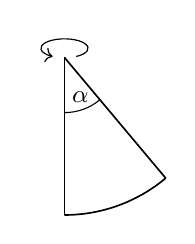
\begin{tikzpicture}[semithick]
		\node[yshift=1mm] {
			\tikz [x=0.12cm,y=0.30cm,line width=.1ex,->,rotate=90] \draw (0,0) arc (-150:150:1 and 1);
		};
		\draw[thin] (0,0) -- ++(270:2cm);
		\draw (0,0) -- ++(310:2cm);
		\draw ([shift=(270:2cm)]0,0) arc (270:310:2cm);
		
		\node[yshift=-5mm,xshift=2mm] {\small$\alpha$};
		\draw[thin] ([shift=(270:7mm)]0,0) arc (270:310:7mm);
	\end{tikzpicture}
	\end{minipage}
	\hspace{0.9cm}$\Rightarrow$\hspace{0.9cm}
	\begin{minipage}{3cm}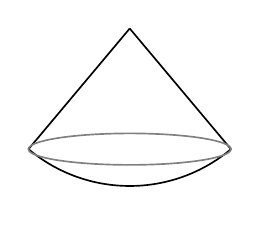
\begin{tikzpicture}[semithick]
		\draw (0,0) -- ++(230:2cm);
		\draw (0,0) -- ++(310:2cm);
		\draw ([shift=(230:2cm)]0,0) arc (230:310:2cm);.
		\draw[gray] ([yshift=-2cm * cos{40}]0,0)ellipse (2cm * sin{40} and 0.2cm);
	\end{tikzpicture}
	\end{minipage}
\end{center}

wtedy: $$\Omega = 2 \pi (1 - \cos (\alpha)) \qquad \Omega \in [0, 4\pi] \Leftrightarrow \Omega \in [0, 12.56\ldots]$$

W przekroju wtedy taki wycinek kóli posiada kąt rozwarcia (który jest także kątem rozwarcia stożka, o tej samej powierzchni stożkowej co ten wycinek kóli): $$\theta = 2 \alpha$$


\subsection{Charakterystyka źródła światła}

\subsubsection{strumień świetlny [lumen, lm]}

Podstawowym parametrem charakteryzującym źródło światła jest emitowany strumień świetlny $\Phi$, którego wartość wyrażana jest w lumenach [lm].

\subsubsection{kąt świecenia}

Drugim parametrem opisującym źródło światła jest kąt bryłowy $\Omega$, w którym emituje ono generowany przez siebie strumień świetlny\footnote{dla uproszenia będziemy zakładać że źródło w całym tym kącie bryłowym emituje promieniowanie równomiernie}.

Kąt świecenia podawany jest jednak zazwyczaj jako kąt rozwarcia stożka świecenia $\theta$, a rzadziej jako kąt bryłowy $\Omega$.
Wiemy jednak że: $\Omega = 2 \pi (1 - \cos (\theta/2))$.

\subsubsection{natężenie strumienia świetlnego [kandela, cd]}

Te dwie wartości pozwalają na obliczenie \strong{światłości} (natężenia strumienia świetlnego) $I$, wyrażanej w kandelach \strong{[cd]}.
$$I = {\Phi \over \Omega} = {\Phi \over 2 \pi (1 - \cos (\theta/2))} \quad \left[{\rm {lm \over sr} = cd}\right]$$

W im większy kąt źródło o danym strumieniu będzie świecić, tym natężenie tego strumienia będzie mniejsze.
Minimum osiągnie dla punktowego źródła izotropowego (świecącego tak samo w każdym kierunku), dla którego:
	$I = {\Phi \over 4 \pi}$ (co odpowiada stożkowi o kącie rozwarcia $\theta = 2 \pi$).


\subsection{Charakterystyka oświetlenia}

W codziennych zastosowaniach zazwyczaj bardziej interesuje nas jasność oświetlenia jakieś powierzchni oddalonej o $r$ od źródła światła niż jasność samego źródła światła.

\subsubsection{natężenie oświetlenia [luks, lx]}

Do określenia jak dobrze oświetlona jest dana powierzchnia stosowane jest natężenie oświetlenia $E$ wyrażane w luksach [lx].
Przy założeniu prostopadłego padania światła na powierzchnię $S$ (czyli np. dla wycinka kóli o promieniu $r$ z źródłem światła w środku):
	$$E = {\Phi \over S} \quad \left[{\rm {lm \over m^2} = lx}\right]$$
Taki wycinek kóli odpowiada kątowi bryłowemu $\Omega = S/r^2$ (z definicji kąta bryłowego), czyli:
	$$E = {\Phi \over \Omega r^2} = {I \over r^2}$$


\subsection{Przykłady źródeł światła}

\subsubsection{świetlówka T8}
$$83 \dots 96 lm/W \qquad\Rightarrow\qquad 6.61 \dots 7.67 cd/W$$

\subsubsection{dioda LED biała 3W}
$$140^\circ, 100lm \quad\Rightarrow\quad \alpha = 70^\circ \quad\Rightarrow\quad$$
$$\Omega = 2 \pi (1 - \cos (70\pi/180)) = 4.134 \rm sr \quad\Rightarrow\quad  24cd \quad\Rightarrow\quad 8 cd/W$$

% Copyright (c) 2021 Robert Ryszard Paciorek <rrp@opcode.eu.org>
% 
% MIT License
% 
% Permission is hereby granted, free of charge, to any person obtaining a copy
% of this software and associated documentation files (the "Software"), to deal
% in the Software without restriction, including without limitation the rights
% to use, copy, modify, merge, publish, distribute, sublicense, and/or sell
% copies of the Software, and to permit persons to whom the Software is
% furnished to do so, subject to the following conditions:
% 
% The above copyright notice and this permission notice shall be included in all
% copies or substantial portions of the Software.
% 
% THE SOFTWARE IS PROVIDED "AS IS", WITHOUT WARRANTY OF ANY KIND, EXPRESS OR
% IMPLIED, INCLUDING BUT NOT LIMITED TO THE WARRANTIES OF MERCHANTABILITY,
% FITNESS FOR A PARTICULAR PURPOSE AND NONINFRINGEMENT. IN NO EVENT SHALL THE
% AUTHORS OR COPYRIGHT HOLDERS BE LIABLE FOR ANY CLAIM, DAMAGES OR OTHER
% LIABILITY, WHETHER IN AN ACTION OF CONTRACT, TORT OR OTHERWISE, ARISING FROM,
% OUT OF OR IN CONNECTION WITH THE SOFTWARE OR THE USE OR OTHER DEALINGS IN THE
% SOFTWARE.

\section{Realizacja instalacji elektrycznych}

Na instalację elektryczną składają się rozdzielnice wraz z zabezpieczeniami i innym osprzętem, okablowanie / oprzewodowanie (kable elektryczne, szynoprzewody), osprzęt elektroinstalacyjny (gniazdka, łączniki, ...).

\subsection{topologie}

Każda instalacja posiada pewną topologię, którą stanowi układ połączeń rozdzielnic i osprzętu oraz odbiorników przy pomocy okablowania / oprzewodowania.
Wyróżnić można kilka podstawowych topologi:
\begin{itemize}
	\item \strong{magistralę} – urządzenia dołączane są do przewodu przebiegającego przez nie, bądź w ich pobliżu (przy pomocy krótkich odgałęzień)
	%\begin{itemize}
		\item \strong{pierścień} – magistrala której końce są ze sobą połączone
	%\end{itemize}
	\item \strong{gwiazdę} – przewody od urządzeń zbiegają się w jednym punkcie i tam następują połączenia.
\end{itemize}
W praktyce na ogół spotyka się różnego rodzaju układy mieszane takie jak:
\begin{itemize}
	\item gwiazda magistral / pierścieni – np. z rozdzielnicy wychodzą 3 magistrale /pierścienie do których przyłączone są kolejne gniazdka
	\item magistrala gwiazd – np. na szynoprzewodzie (stanowiącym magistralę) zamontowane są skrzynki odpływowe z których wychodzą obwody do zasilania odbiorników (w układzie gwiazdy)
	\item gwiazda wielokrotna - np. z głównej rozdzielnicy wychodzi 5 obwodów, każdy przeznaczony do zasilania kolejnej rozdzielnicy
\end{itemize}\nopagebreak[4]%
i ich kombinacje.\pagebreak[1]

Układ z rozdzielnią główną oraz podrozdzielnicami umieszczonymi na obiekcie jest bardzo popularny w przemyśle i obiektach komercyjnych (biura, hotele, obiekty handlowe, itd.), natomiast (co trochę dziwne) nie jest sotowany nawet w dużych domach jednorodzinnych (gdzie pojedyncza rozdzielnica potrafi przekraczać 400 modułów).

Zaletą magistral jest mniejsza ilość przewodu potrzebnego do ich wykonania oraz mniejsza ilość obwodów pojawiających się w rozdzielnicy.
Zaletą gwiazdy jest możliwość sterowania dowolnym z obwodów z punktu centralnego (rozdzielnicy) i stosunkowo łatwej rekonfiguracji
	(np. podzielenia obwodu gniazd złożonego z kilku/kilkunastu przewodów wprowadzonych do rozdzielni zakończonych gniazdami, a podłączonych do jednego zabezpieczenia na kilka niezależnych obwodów podłączonych do osobnych zabezpieczeń).
Często też stosowane są rozwiązania pośrednie czyli (ze względu na sterowanie – \textit{inteligentny budynek} okablowanie wykonywane jest w gwiazdę,
	ale nie dotyczy to każdego gniazdka (bo nie planujemy sterowania nimi) i do rozdzielni trafiają przewody od grup gniazdek łączonych magistralą (np. 1 lub 2 grupy na pomieszczenie).

Oczywiście możliwe jest też wykonanie sterowania w układzie nie będącym gwiazdą (czyli np. sterowania indywidualnego każdym gniazdkiem w grupie spiętej na jednej magistrali) – wymaga to zastosowania rozproszonych modułów sterujących (np. zlokalizowanych w każdym z gniazdek).

\subsection{trasy kablowe}

Instalacje elektryczne mogą być prowadzone/montowane na dwa sposoby:
\begin{itemize}
	\item po wierzchu
	\item ukryte w ścianach, podłogach, itd (instalacje „podtynkowe”)
\end{itemize}

Zasadniczymi różnicami pomiędzy tymi sposobami prowadzenia instalacji jest łatwość ich prowadzenia i późniejszej modyfikacji vs względy estetyczne.
Przy czym warto tutaj zaznaczyć iż ładnie wykonana imnstalacja „natynkowa” jest estetyczna i dla niektórych stylów urządzania wnętrz może być wręcz atutem.

Instalacje prowadzone po wierzchu dominują w zastosowaniach przemysłowych, natomiast te ukryte w mieszkaniowych.
Funkcjonują także rozwiązania „kompromisowe”, często spotykane w obiektach komercyjnych (biura, obiekty handlowe, starsze rozwiązania serwerowni\footnote{Obecnie serwerownie realizowane są coraz częściej „po wierzchu”, jak typowy przemysł.}
	– ukrycie instalacji nad sufitami kasetonowymi, pod podłogami podnoszonymi, zastosowanie plastikowych kanałów instalacyjnych na których bezpośrednio montowany jest osprzęt elektryczny.

Pośród instalacji prowadzonych na wierzchu można wyróżnić kilka sposobów ich prowadzenia (mogą być one też mieszane w ramach danej instalacji):
\begin{itemize}
	\item szynoprzewody
	\item koryta metalowe (pełne, perforowane lub siatkowe) i drabiny kablowe
	\item rurki plastikowe
	\item przewód montowany bezpośrednio na uchwytach kablowych
	\item plastikowe korytka i kanały instalacyjne
\end{itemize}

Należy zachować odległość pomiędzy trasami w których prowadzone jest wysokoprądowe okablowanie zasilające od tras w których prowadzone jest „miedziane” (nie światłowodowe) okablowanie sterujące, telekomunikacyjne lub inne okablowanie „niskoprądowe”.

\begin{figure}[ht!]
\begin{center}\begin{tabular}{cc}
\includegraphics[width=0.47\textwidth]{elektryka/Cabtray_11.jpg} & % https://commons.wikimedia.org/wiki/File:Cabtray_11.jpg  Leotard, CC-0
\includegraphics[width=0.47\textwidth]{elektryka/Cabtray_10.jpg} % https://commons.wikimedia.org/wiki/File:Cabtray_10.JPG  Leotard, CC-0
\\
koryta stalowe perforowane i drabiny kablowe &
koryta siatkowe
\end{tabular}\end{center}

\begin{center}\begin{tabular}{ccc}
\includegraphics[trim={0 14cm 0 0},clip,width=0.47\textwidth]{elektryka/OrganizedElectricalWiring.jpg} & % https://commons.wikimedia.org/wiki/File:OrganizedElectricalWiring.jpg  KVDP, PD
\includegraphics[trim={6cm 0 2cm 0},clip,width=0.176\textwidth]{elektryka/IMG_20210731_145157.jpg} &
\includegraphics[trim={10cm 0 50cm 0},clip,width=0.263\textwidth]{elektryka/Cabtray_03.jpg} % https://commons.wikimedia.org/wiki/File:Cabtray_03.JPG  Leotard, CC-0
\\
koryta stalowe pełne &
instalacja natynkowa &
kanał instalacyjny PCV
\\
&
bez rurek &
z osprzętem 45x45mm
\end{tabular}\end{center}

\begin{center}\begin{tabular}{cc}
\includegraphics[width=0.47\textwidth]{elektryka/szynoprzewody.jpg} &
\\
szynoprzewody z kasetami dystrybucyjnymi &
\\
powieszone na konstrukcji z ceowników montażowych &
\end{tabular}\end{center}
\end{figure}

\subsubsection{montaż tras kablowych}

Elementy budujące „natynkowe” trasy kablowe, takie jak rurki, czy koryta mogą być montowane bezpośrednio do ściany.
Często jednak stosuje się dodatkowe konstrukcje służące ich zamocowaniu – zwłaszcza w przypadku koryt metalowych i szynoprzewodów.
Pozwalają one na montaż koryta do ściany lub sufitu z zachowaniem „orientacji” koryta w przestrzeni,
	czyli bez jego obracania, tak aby kable leżały na jego dnie a nie boku (dzięki czemu nie będą wypadać i nie ma potrzeby stosowania np. pokrywy do koryta).
Koryta mogą być mocowane do ścian przy użyciu różnego rodzaju wsporników, podwieszane do sufitu za pomocą szpilek,
	czy też montowane zarówno do ścian jak i sufitów na bardziej rozbudowanych konstrukcjach głównie z ceowników montażowych\footnote{
		Ceownik montażowy jest to profil (zazwyczaj stalowy) przypominający w przekroju literę C / U, gdzie boczne ścianki sa lekko zagięte do środka.
		Takie ukształtowanie zapewnia większą sztywność oraz pozwala na montaż elementów do „wnętrza” ceownika z użyciem nakrętek rombowych.
	}.
Zaletą zastosowania konstrukcji z ceowników w stosunku co do podwieszenia na szpilkach jest zapewnienie większej sztywności całej trasie kablowej.
Jest to szczególnie istotne przy montażu szynoprzewodów, które będą obciążane jeszcze dodatkowo skrzynkami odpływowymi –
	zwykłe ich podwieszenie na szpilach nie zapewni sztywności i pozornie sztywne szynoprzeody zaczną się skręcać i chwiać.

\begin{figure}[ht!]
\begin{center}\begin{tabular}{ccc}
\includegraphics[height=5.5cm]{elektryka/ceowniki1.jpg} &
\includegraphics[height=5.5cm]{elektryka/ceowniki2.jpg} &
\includegraphics[height=5.5cm]{elektryka/ceowniki3.jpg}
\\
ceownik montażowy wraz z elementem &
wspornik zamocowany &
wykorzystanie perforacji 
\\
montowanym z użyciem nakrętki rombowej &
do ceownika &
ceownika do montażu
\end{tabular}\end{center}
\end{figure}

\subsection{rozdzielnice}

Przy planowaniu, projektowaniu rozdzielnic najistotniejsze jest zapewnienie odpowiednio dużo miejsca w rozdzielnicy – zarówno dla zmieszczenia samej aparatury i okablowania, jak też komfortu wykonywania prac serwisowych (dostęp do wszystkich elementów, zacisków, itd) oraz ew. rozbudowy czy modyfikacji. Przy wykonywaniu (prefabrykacji, montażu, kablowaniu) rozdzielnicy istotna jest estetyka i przejrzystość, która ułatwia późniejsze prace serwisowe.

Istnieje wiele rozwiązań konstrukcyjnych dla rozdzielnic elektrycznych, często nawet pojedynczy producent posiada kilka (niekompatybilnych ze sobą) takich systemów.
Konkretne rozwiązanie konstrukcyjne powinno być dobrane z uwzględnieniem tego co w danej rozdzielnicy będzie się znajdować i jak jest to montowane (szyna DIN, płyta montażowa, rack 19", ...).
Warto jednak pamiętać że na ogół nie wszystko musi się znaleźć w jednej obudowie i czasami lepiej jest zastosować osobną rozdzielnicę modułową i np. osobną obudowę z płytą montażową na pojedynczy duży aparat.
Albo osobną rozdzielnicę elektryczną i osobną szafkę rack na montaż kilku paneli krosowych i switcha.
Istotne jest dobre wykorzystanie miejsca i wykonanie zapewniające wygodę obsługi i serwisu.
Warto aby rozdzielnica zapewniała odpowiednią głębokość, ale raczej należy unikać montażu na kilku głębokościach na tej samej wysokości (pozwala to zmieścić więcej urządzeń, ale utrudnia dostęp).

\subsection{standardy}

\subsubsection{szyna DIN}

\begin{wrapfigure}{r}{2.7cm} %
\vspace{-0.8cm}\includegraphics[trim={0cm 0 0.2cm 0},clip,width=2.5cm]{img/elektryka/DIN-rail-dimensions}\vspace{-0.5cm} % https://commons.wikimedia.org/wiki/File:DIN-rail-dimensions.svg  Markus Kuhn as Public Domain
\end{wrapfigure}

Standard szyny \href{https://en.wikipedia.org/wiki/DIN_rail}{montażowej DIN} określa kilka rodzajów szyn.
Najpopularniejszą z nich jest szyna TH-35, szyli szyna o szerokości 35mm z blachy o grubości 1mm, zagłębiona w środkowej części na szerokości 25mm o co 7.5 mm lub 15mm (zależnie od wariantu).

Sam standard szyny nie określa niczego więcej.
W ogólności kształt obudów montowanych na szynę DIN nie jest zestandaryzowany (spotykane sa np. obudowy o wysokości kilkunastu cm).

Natomiast jest określony kształt obudów aparatury modułowej montowanej na szynę DIN.
Typowy moduł nie przekracza 47mm głębokości od szyny TH do części zakrywanej panelem przednim obudowy, 70mm głębokości od szyny TH do frontu aparatu, który liczy 45 mm wysokości.
Zapewnia to że większość aparatury modułowej da się zainstalować nawet w płytkiej rozdzielnicy bez możliwości regulacji głębokości szyn.
Natomiast szerokość przypadająca na jeden biegun zasilania wynosi 17.5mm, co pozwala na stosowanie standardowych szyn łączeniowych do aparatów.

Typowo długość szyny (szerokość zamontowanych na niej urządzeń) określa się właśnie w modułach o szerokości 17.5mm (±0.5mm).\footnote{Stosowane są także urządzenia o szerokości mniejszej niż jeden moduł – np. styki pomocnicze, złączki kablowe.}
Przez to, że standardowy jednopolowy wyłącznik nadprądowy posiada właśnie szerokość 1 modułu, to ilość modułów daje pewne wyobrażenie o wielkości rozdzielnicy.


\subsubsection{rack 19"}

Standard \href{https://en.wikipedia.org/wiki/19-inch_rack}{rack 19"} wywodzi się z telekomunikacji i jest powszechnie stosowany w rozwiązaniach IT.
Bywa jednak stosowany w zastosowaniach elektrycznych.
Stosowane są moduły wysokości 3U wyposażone w szynę DIN TH-35 do montażu aparatury elektrycznej w ramie rack 19".
Stosowane są także adaptery do montażu (odpowiednio krótkich) urządzeń rack 19" w (dostatecznie szerokich) rozdzielnicach elektrycznych.

Standard rack 19" (\href{https://www.server-racks.com/eia-310.html}{EIA-310}) określa jedynie podstawowe parametry montażowe dla płyt czołowych:
\begin{itemize}
	\item wymiary poziome:
	\begin{itemize}
		\item odległość pomiędzy wewnętrznymi krawędziami szyn montażowych (maksymalną szerokość obudowy montowanego urządzenia): 17~3/4" (450mm)
		\item ogległość pomiędzy środkami otworów montażowych: 18~5/16" (465.1mm)
		\item szerokość płyty czołowej urządzenia obejmującą otwory montażowe: 19" (482.6mm)
	\end{itemize}
\end{itemize}

~\vspace{-32pt}
\begin{wrapfigure}{r}{5.5cm}%
\vspace{-0.4cm}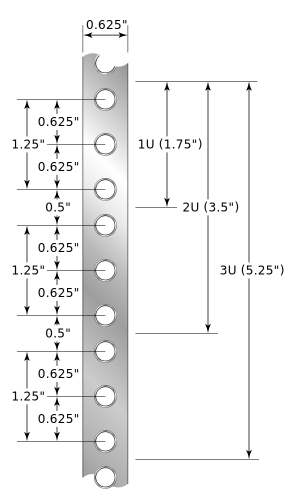
\includegraphics[width=5.3cm]{img/elektryka/Server_rack_rail_dimensions}\vspace{-2.6cm} % https://commons.wikimedia.org/wiki/File:Server_rack_rail_dimensions.svg  Sakurambo as Public Domain
\end{wrapfigure}

\begin{itemize}
	\item wymiary pionowe:
	\begin{itemize}
		\item jednostkę wysokości urządzenia \strong{\href{https://en.wikipedia.org/wiki/Rack_unit}{1U}}=1 3/4" (44.45mm)
		\item odległości środków trzech otworów montażowych w ramach każdego „U”:
			\begin{itemize}
				\item pierwszy otwór: 1/4" (6.35mm) od krawędzi
				\item środkowy otwór: 5/8" (7.95mm) od środka pierwszego
				\item trzeci otwór: 5/8" (7.95mm) od środka środkowego i 1/4" (6.35mm) od krawędzi
			\end{itemize}
			co razem daje 1 3/4" czyli jednostkę wysokości
	\end{itemize}
\end{itemize}

Standard pozwala także na stosowanie różnego typu otworów w profilu montażowym – gwintowane (3/16", 7/32", M5, lub M6), okrągłe niegwintowane lub kwadratowe (3/8" x 3/8", pozwalające na montaż nakrętki typu \textit{\href{https://www.server-racks.com/what-is-a-cagenut.html}{cage nut}}).

Natomiast nie określa:
\begin{itemize}
	\item głębokość szafy ani montowanego sprzętu
	\item formy ani sposobu mocowania jakichkolwiek dodatkowych podparć (dla długich urządzeń), prowadnic kulkowych, itp.
	\item \href{https://www.server-racks.com/rack-upright-shape.html}{kształtu profili} z otworami montażowymi
	\item ilości profili montażowych (czy występują środkowe / tylne)
	\item jakichkolwiek innych aspektów konstrukcyjnych szafy / stojaka (także tego czy to ma być zamknięta szafa czy w pełni otwarty stojak)
\end{itemize}

Można spotkać się także z odmianą 10" oraz 9.5" (half-rack). Ta druga pozwala na montaż dwóch urządzeń obok siebie w standardowym racku 19".


\copyrightFooter{
	© Robert Ryszard Paciorek <rrp@opcode.eu.org>, 2021.\\
	Wykorzystano grafiki należące do domeny publicznej.\\
	Kopiowanie, modyfikowanie i redystrybucja dozwolone pod warunkiem zachowania informacji o autorach.
}
\end{document}
